
\documentclass[a4paper,UKenglish,cleveref, autoref, thm-restate]{lipics-v2021}

\bibliographystyle{plainurl}% the mandatory bibstyle
\usepackage{booktabs}   %% For formal tables:
                        %% http://ctan.org/pkg/booktabs
\usepackage{subcaption} %% For complex figures with subfigures/subcaptions
                        %% http://ctan.org/pkg/subcaption

\usepackage{mathtools}
\usepackage{todonotes}
\usepackage{microtype}

\usepackage{complexity}
\usepackage{amsmath}
\usepackage{dsfont}

\usepackage{stmaryrd}
\usepackage{MnSymbol}
\usepackage{graphicx}




\newcommand{\problemx}[3]{
	\vspace{0.2cm}
\par\noindent\underline{\sc#1}\par\nobreak\vskip.2\baselineskip
\begingroup\clubpenalty10000\widowpenalty10000
\setbox0\hbox{\bf INPUT:\ }\setbox1\hbox{\bf QUESTION:\ }
\dimen0=\wd0\ifnum\wd1>\dimen0\dimen0=\wd1\fi
\vskip-\parskip\noindent
\hbox to\dimen0{\box0\hfil}\hangindent\dimen0\hangafter1\ignorespaces#2\par
\vskip-\parskip\noindent
\hbox to\dimen0{\box1\hfil}\hangindent\dimen0\hangafter1\ignorespaces#3\par
\endgroup
	\vspace{-0.2cm}
}

\newcounter{claimcounter}
\setcounter{claimcounter}{0}
\newtheorem{subclaim}{Subclaim}{}
\newtheorem*{theorem*}{Theorem}

\makeatletter

\usepackage{ textcomp } 

\usepackage{stmaryrd}
\usepackage{MnSymbol}
\usepackage{graphicx}

\usepackage{wrapfig}


\newcommand\sg[1]{\todo[inline,size=\scriptsize]{#1 - \textbf{Stefan}}}
\newcommand\mh[1]{\todo[inline,size=\scriptsize]{#1 - \textbf{Mathieu}}}
\newcommand\sgchanged[1]{{\color{red}{'1}}}
\newcommand\mhchanged[1]{{\color{blue}{'1}}}


\renewcommand{\A}{\mathcal{A}}
\newcommand{\B}{\mathcal{B}}
\renewcommand{\C}{\mathcal{C}}
\newcommand{\T}{\mathcal{T}}
\renewcommand{\G}{\mathcal{G}}
\renewcommand{\O}{\mathcal{O}}
\renewcommand{\R}{\mathbb{R}}
\renewcommand{\H}{\mathcal{H}}
\newcommand{\Z}{\mathbb{Z}}
\newcommand{\N}{\mathbb{N}}
\newcommand{\Time}{\mathbb{T}}
\newcommand{\Const}{\mathsf{Consts}}
\newcommand{\Conf}{\mathsf{Conf}}
\newcommand{\PTA}{\textsc{PTA}}
\newcommand{\MSO}{\textsc{MSO}}


\renewcommand{\poly}{\mathrm{poly}}

\newcommand{\Op}{\mathsf{Op}}
\newcommand{\win}{\textsc{Win}}



\newcommand{\semi}[1]{\xRightarrow{'1}}




\title{Parity games in pushdown systems with parameters} 

\titlerunning{Parity games in pushdown systems with parameters} 

% \author{Stefan G\"oller}{University of Kassel \and School of Electrical Engineering and Computer Science \and Kassel, Germany }{stefan.goeller@uni-kassel.de}{}{The author was supported by the Agence Nationale de la Recherche grant no.  ANR-17-CE40-0010.}
\author{Mathieu Hilaire}{Université Paris-Saclay\and
CNRS\and
ENS Paris-Saclay\and
Laboratoire Méthodes Formelles (LMF)\and
Gif-sur-Yvette, France
}{hilaire@lsv.fr}{}{This work was partly done while the author was supported by the 
Agence Nationale de la Recherche grant no.  ANR-17-CE40-0010.}

\authorrunning{M. Hilaire} 

\Copyright{M. Hilaire} 

%\ccsdesc[500]{Theory of computation~Timed and hybrid models}
%\ccsdesc{Theory of computation~Automata over infinite objects}
\ccsdesc[500]{Theory of computation~Automata extensions}

\keywords{Parity Games, Computational Complexity, Pushdown systems, Pebble Alternating Two Way Automata}



\category{} 

\relatedversion{}
% \relatedversiondetails{Full Version}{}

\acknowledgements{The author would like to thank Benedikt Bollig and Stefan G\"oller for helpful discussions and feedback.}


\ArticleNo{70}
\begin{document}

\maketitle


\begin{abstract}
	We investigate the decidability and complexity of
	parity games over an extension of pushdown systems.
	More specifically, we consider parameters pushdown systems, in
	which parameters can be instantiated to some word over a stack alphabet,
	and compared against the current stack content.
	We determine decidability of the problem, and provide a nonelementary lower bound. 
\end{abstract}

\section{Introduction}

\subsubsection*{Background}


{\bf Context}
Stack-based automata \textcolor{red}{pourquoi ne pas commencer directement avec lesPushdown systems ?}are a popular formalism for modeling the sequential behavior of computer programs. 
Pushdown systems \textcolor{red}{or stack-automata ?}are probably the most studied models of stack-based automata.
\textcolor{red}{inutile: They are
finite automata 
 extended with a stack that can be manipulated by pushing or popping stack symbols from some finite set, and can use the top of the stack to decide which transition to take next.}
\textcolor{blue}{ok je comprends que tu signales la différence mais c'est trop détaillé pour cet endroit du texte: To underline the fact that we are concerned with the graph of configurations and not the language recognized, we use the name pushdown system rather than pushdown automaton.}

{\bf Games on pushdown systems}Pushdown systems can be used to model the behavior of recursive programs and,
as a result, a variety of 
 program analysis questions can be reduced to decision problems for games on pushdown systems.
They have applications for instance in inter-procedural control-flow analysis of recursive programs \cite{esparza1999automata, reps2005weighted}.





Two player games can be used in particular to
 represent the
interaction of a program with some environment, with the first player representing the program while the second player represents the environment. A winning condition then expresses a property required to hold however the environment behaves. Finding a winning strategy for the first player
thus provides some way 
 to ensure that the desired 
property, as expressed by the winning condition,
always holds \cite{arnold2003games}.


Games on the graphs of pushdown systems have been extensively studied.
It is known in particular from \cite{walukiewicz1996pushdown} that deciding the winner of a parity game on a graph of a pushdown system is an ${\sf EXPTIME}$-complete problem.
Several generalizations of the pushdown systems 
have been studied in depths, including
tree-pushdown systems \cite{guessarian1983pushdown}, ordered
multi-pushdown systems \cite{breveglieri1996multi, atig2012model}, annotated higher-order pushdown systems \cite{maslov1976multilevel, broadbent2012saturation}, and
strongly normed multi-pushdown systems \cite{czerwinski2012reachability}.



{\bf Parametric pushdown automata or systems ?}
 Parametric pushdown automata provide a  formalism to
reason about 
recursive programs
making use of parametric constraints.
% Here, the stack can additionally be compared against parameters that can take unspecified word values. 
Recently, different variants of parametric pushdown automata have been introduced in the literature 
% [Hague’11]=[20], [Esparza, Ganty, Majumdar’13]=[15]
\cite{hague2011parameterised, esparza2016parameterized, fortin2017model} 
% In this work, following [21,20,15,27,12], we consider parametric pushdown systems
however as
parameterized asynchronous shared-memory systems.
These systems consist of a leader pushdown automaton
and arbitrarily many identical contributor pushdown automata, communicating via a shared memory
in the form of a register which can take finitely many values.
This variant have been shown to have applications
to the dataflow analysis of concurrent programs \cite{kahlon2008parameterization}. 
We consider here a different approach to extending pushdown automata with parameters, by allowing them to test equality of the stack content against parameters.
% Pushdown systems which can test the stack content against regular-expressions are equivalent to pushdown systems, so pushdown systems which can test the stack content against specific words are too.
Perhaps a similar model consists in 
pushdown automata 
with transitions that are conditioned by regular conditions on their stack content, which
can in particular
test the
stack content against
specific words. 
They can be used to ensure that some word over the stack alphabet appears in the configurations of a run, but only for a specific value (or, rather, specific regular languages),
and have \textcolor{red}{ phrases trop longues}
been used to establish that CTL$^*$ model checking remains decidable
when the formulas are allowed to include regular predicates on the stack content,
and to obtain 
model checking algorithms for LTL and CTL$^*$ model checking
for
pushdown automata \cite{finkel1997direct}.
Pushdown automata 
%with regularity condition on the stack
with transitions that are conditioned by regular conditions on their stack content
can be viewed as
a special case of stack automata as seen in \cite{hopcroft1969formal}.
Instead
of checking the stack content against regular conditions, or, in a more limited manner,
against specified word values,
we consider
checks against unspecified word values that can be instantiated using parameters.
This allows for example to ensure equality between two stack contents appearing in two distincts configurations in a run.

{\bf Extensions of  pushdown automata/systems ?}
Extensions of pushdown automata with storage for later comparisons
have been introduced for instance as register pushdown automata. 
Such automata possess registers in addition to their stack, and can keep data values in both.
Register pushdown automata have been shown to have applications for malware detection and XML schema checking \cite{senda2021forward, senda2021ltl}. 
In theory, since registers can be unfilled and later be filled again an unbounded number of times, the number of different data values a pushdown register automata can store in its registers in a run is unbounded.  
In \cite{murawski2017reachability} it was shown however that a register pushdown automaton can
only really ``remember'' at most  $3r$ data values, where $r$ is the number of registers,
% Even though pushdown register automata have no bound on the number of elements of the alphabet that they can store at any instant, over the course of a run they can really “remember” at most 3r of them, 
i.e. for any run of a register pushdown automaton with $r$ registers there exists an equivalent run %, i.e.
 with the same initial and final configurations, but in which every configuration contains register assignments drawn from only $3r$ elements. This 
 %can 
 leads to
 the
  question
  of
   how useful the ability to unfill and later refill registers really is compared to a model that would only specify valuations once.



% Hence we propose in this paper to extend pushdown systems with a set of  parameters.
%
% Compared to pebble word automata, instead of using pebbles
% as markings on their input, pebble pushdown systems have the ability to lift or drop pebbles
% on their universe of stack contents. Dropping a pebble records the current stack content with an available pebble until it is lifted. Lifting a pebble then makes it available again.


% A pebble automaton is a two-way finite state automaton that uses a fixed, finite number of
% pebbles that it can drop on, and lift from 
% words, using them as markers.
% Pebble automata recognize regular languages only, provided the life times of the pebbles, i.e. the times between dropping a pebble and lifting it again, are properly nested
% \cite{globerman1996complexity, engelfriet1999tree}.
% Automata with nested pebbles were also introduced for tree-walking automata. 
% It is known that tree-walking automata do not recognize all regular tree languages \cite{bojanczyk2008tree}, the main trouble being that the tree-walking automata get lost rather easily.
% Using pebbles is a remedy against getting lost along a tree, but  the unrestricted use of pebbles leads to a class of tree languages much larger than the regular tree languages, in fact to all tree languages in $\NSPACE(log ~ n)$.
% Thus, in both pebble word automata and pebble tree-walking automata, the placement of the pebble follows a strict stack discipline, and our model will follow this strict stack discipline too.
%
%
% One motivation to the study of pebble pushdown systems is their ability to compare a stack content against some later stack content.
% Similar type of storage for later comparison has already been used for instance in register pushdown systems. Introduced in \cite{murawski2017reachability}  as an extension of pushdown systems that can keep data values in a set of registers and a stack, register pushdown systems enable manipulation of data values from an infinite domain, and have applications for instance for malware detection and XML schema checking \cite{senda2021forward, senda2021ltl}.




Another closely related formalism is that of alternating tree automata with nested pebbles%, as we consider in more details in Section 4
. The approach of extending tree automata with pebbles was used in \cite{milo2000typechecking} to show that the XML typechecking problem is decidable, and in \cite{karhumaki2012jewels} to recognize first-order logic on trees. In both cases however, the input trees considered are finite, while 
simulation of plays in parametric pushdown graphs
requires the use of pebble alternating tree automata working on infinite trees
since the stack of a pushdown system is in general unbounded.



The aim of the present paper is to study the decidability and complexity of
deciding
the winner of a parity game on a graph of a pushdown system with  
parameters.


 \iffalse
 
 
We provide formal definitions of parametric pushdown automata, parametric pushdown reachability games
and parametric pushdown parity games in Section~\ref{section def ppda}. We give an overview of our contribution in Section~\ref{contribution ppda}. The contribution consists in
proving parametric pushdown reachability games
and parametric pushdown parity games belong to $(n+1)$-$\EXP$ in case the number of parameters
$n$ is fixed,
and providing a nonelementary lower bound for parametric pushdown reachability games in general.
We provide the proof of our result, which stretches along 
Section~\ref{lower bound PDA},
Section~\ref{pebbles},
% Section~\ref{ATWA and PATWA}, and
Section~\ref{section HPDA}.
In Section~\ref{discuss ppda} we close the chapter with a discussion about the methods used, with some directions for future work.
\fi

\subsubsection*{Our contributions}


Our main result consists in
proving parametric pushdown reachability games
and parametric pushdown parity games belong to $(n+1)$-$\EXP$ in case the number of parameters
$n$ is fixed,
and providing a nonelementary lower bound for parametric pushdown reachability games in general.



	For the nonelementary lower bound,
we reduce the $\FO$ satisfiability problem on words, known to be nonelementary
from \cite{Sto74}, to the
problem of deciding whether a player has a winning strategy for parametric pushdown reachability games. 

	For the upper bound, we start by replacing parameters by pebbles acting as registers, leading to a more general model, pebble pushdown automata.
 We then show that higher-order pushdown automata parity games can be used to solve parity games on
 the transition systems of pebble pushdown automata,
using one additional stack level for each pebble.
 Since solving parity games on higher-order pushdown automata with level $n$ stack is $n$-$\EXP$-complete \cite{ Cach03, cachat2007complexity}, this provides an $(n+1)$-$\EXP$ upper bound for solving parametric parity games on parametric pushdown automata with $n$ parameters.



\subsubsection*{Overview}

In Section 2, we provide general notations and preliminary definitions. 
Section 3 will deal with the introduction of  parametric pushdown games.
% Section 4 is devoted to using pebble alternating tree automata with parity acceptance condition to solve parametric pushdown system parity games. We leave the proof of decidability itself  for Section 5.
Section 4 is Reduction to higher-order pushdown automata
Section 5 at last shows a nonelementary lower bound for the problem.




\section{Definitions}


\newcommand{\LCM}{\mathsf{LCM}}
\newcommand{\LOGSPACE}{\mathsf{LOGSPACE}}
\renewcommand{\MSO}{\mathsf{MSO}}
\newcommand{\SO}{\mathsf{SO}}

By $\Z $ we denote the {\em integers} and by $\N=\{0,1,\ldots\}$ we denote the {\em naturals}.
% For every $a,b\in\Z$ with $a\leq b$ we define $[a,b]=\{k\in\Z\mid a\leq k\leq b\}$.
% For every $n\geq 1$ we define $n\Z=\{n\cdot z\mid z\in\Z\}$.
% For every number $n\in\N$ we define $\log(n)=\min\{i+1\mid i\in\N, n\leq 2^i\}$, which is the smallest number of bits necessary to write down $n$ in binary.
For every finite alphabet $A$, $A^*$ is the set of finite
words with letters in  $A$, $A^\omega$ is the set of infinite words with letters in $A$, and
%by
 $A^\infty = A^\omega \cup A^*$. We denote the empty word in $A^*$ by $\epsilon$.
%For all $a\in A$ and all $w\in A^*$ let $|w|_a$ denote the number of occurrences of the letter $a$ in $w$.
%
% For every finite set $M\subset\N\setminus\{0\}$ let $\LCM(M)=\min\{n\geq 1\mid \forall m\in M\setminus\{0\}: m|n\}$ denote the least common multiple of the elements in $M$. 
% For any $j \in \N$ let $\LCM(j)=\LCM([1,j])$ denote the least common multiple of the numbers $\{1,\ldots,j\}$.

 For any two sets $X$ and $S$, let $X^S$ denote the set of all functions from $S$ to $X$.
For any set $S$ let 
%$\mathscr{P}(S) = \{ X \mid X \subseteq S \}$
$\mathcal{P}(S) = \{ X \mid X \subseteq S \}$
denote the power set of $S$.
%
A {\em partial function} $f$ from a set $X$ to a set $Y$ is a function defined on a subset $C$ of $X$ (possibly $X$ itself) with output values in $Y$. We extend the domain of a partial function to the whole set
by considering it as returning the bottom element $\bot$ when it is undefined.




A {\em graph} $G=(V,E)$ is a finite set of graph vertices $V$ with a set of graph edges $E \subseteq V \times V$. 
% Two graphs $G = (V,E)$ and $G'=(V',E')$ with sets of graph vertices $V=V'=V_n=\{1,2,...,n\}$ are said to be {\em isomorphic} if there is a permutation $\rho$ of $V_n$ such that $(u,v)$ is in the set of graph edges $E$ iff $(\rho(u),\rho(v))$ is in the set of graph edges $E'$.
%%%
%
For any set $V$, and a given infinite sequence $\pi = v_0 v_1 \ldots \in V^\omega$ of elements of $V$, we define the set 
$\text{\textit{Inf}}(\pi)$ of elements occurring infinitely often in $\pi$ as
$\text{\textit{Inf}}(\pi) = \{ v \in V \mid \forall i, \exists j > i, ~ v_j = v \}$. 



		\iffalse


\subsection{Logics}

We now briefly review some standard definitions from mathematical logic.

\begin{samepage}
\begin{definition}
 A {\em vocabulary} $\tau$ is a set of relational symbols (denoted $P_1, P_2, \ldots $), each of which has a specified
 arity. A symbol $P \in \tau$ is called monadic if its arity is one, i.e., if it is used to
 denote sets.
%
A {\em $\tau$-structure} %(also called a {\em model})
%
$$ \mathfrak{A} = (A,	( P^{\mathfrak{A}} )_{P \in \tau})$$
%
consists of a set $A$ together with an interpretation of
 each $k$-ary relational symbol $P$ from $\tau$ as a $k$-ary relation on $A$; that is, a
set $P^{\mathfrak{A}} \subseteq A^k$.
% A structure $\mathfrak{A}$ is called finite if $A$ and $\sigma$ are finite sets. 
% The {\em universe} of a structure is typically denoted by a Roman letter corresponding to the name of the structure; that is, the universe of $\mathfrak{A}$ is the set $A$, the universe of $\mathfrak{B}$ is $B$, and so on. We shall also occasionally write $a \in \mathfrak{A}$ instead of $a \in A$.\newline
%
\end{definition}
\end{samepage}


%\noindent As an illustration, if $\tau$ consists of a single relational symbol $E$ of arity $2$, graphs are possible $\tau$-structures. 




% Next, we define the  monadic second-order logic, or $\MSO$.

Next, we define monadic second-order formulas over a vocabulary $\tau$, or $\MSO[\tau]$ for short. %We define free variables, and the semantics of $\MSO(\tau)$ formulas.

\begin{samepage}
\begin{definition}\label{MSO}
We assume countably infinite sets of first-order variables {\em Var}
and of second-order variables {\em VAR}. First-order variables
will be typically denoted by $x, y, z, \ldots,$ with subscripts and superscripts,
whereas second-order variables will be typically denoted by $X, Y, Z, \ldots ,$
using subscripts and superscripts as well. We
inductively define %terms and 
formulas of the monadic second-order logic
over vocabulary $\tau$ %as follows: 
by the grammar:
$$ \phi :=  P(x_1 , \ldots , x_k) \mid x_1 = x_2 \mid X(x) 
		\mid \phi \vee \phi \mid \phi \wedge \phi \mid \neg \phi 
		\mid \exists x ~ \phi \mid  \forall x ~ \phi
		\mid \exists X ~ \phi \mid  \forall X ~ \phi		$$
where $P \in \tau$ is a $k$-ary relational symbol, $X \in \text{VAR}$, and $x, x_1, \ldots, x_k \in \text{Var}$.
\end{definition}
\end{samepage}

A formula that does not use existential ($\exists$) nor universal ($\forall$) quantifiers
is called {\em quantifier-free}.
%
% Given a set of formulas $S$, formulas constructed from formulas in $S$ using only the Boolean connectives $\vee$, $\wedge$, and $\neg$ are called {\em Boolean combinations} of formulas in $S$.
%
We shall use the standard shorthand $\phi  \to \psi $ for $ \neg \phi \vee \psi $ 
and $\phi \leftrightarrow \psi $ for
$(\phi  \to \psi ) \wedge (\psi  \to \phi )$. 


If $\overrightarrow{x}$ is the tuple of all the free first-order variables of $\phi$,
and $\overrightarrow{X}$ is the tuple of all the free second-order variables of $\phi$ 
we write $\phi(\overrightarrow{x},\overrightarrow{X})$. A {\em sentence}
is a formula without free variables. We use the standard semantic of $\MSO$,
see Appendix~\ref{MSO appendix} for a more thorough induction over the formula.\\





Concerning the logic $\MSO$, we are interested in the following decision problem.

\problemx{$\MSO[\tau]$ model-checking}
{A $\tau$-structure $\mathfrak{A}$ and a $\MSO[\tau]$-sentence $\phi$.}
{Does $\mathfrak{A} \models \phi $ ?\newline}


\textcolor{black}{We define the problem in a general abstract manner, instead of focusing on particular representation for the input, since we will consider many structures of infinite size.}



{\em First-order logic over a vocabulary $\tau$} ($\FO[\tau]$ for short) is the fragment of $\MSO$ which is restricted to first-order quantifiers and variables: quantification is permitted only over individuals, and no second-order variables are used. 



		\fi



%ù \subsection{Games}


A {\em game} is composed of an arena and a winning condition.
We will first study
arenas and
 then introduce common winning conditions that will be of interest to us.

% \subsubsection{Arenas}

\begin{samepage}
An {\em arena} is a tuple $A=(S_0, S_1,{\rightarrow})$  which is composed of
\begin{itemize}
	\item two  disjoint  sets of configurations, $S_0$ and $S_1$, %respectively associated with player $0$ and $1$, 
	whose disjoint union $S_0 \cup S_1$ we denote by $S$, and
	\item a relation of %labeled 
		transitions
	 ${\rightarrow} \subseteq S \times %\Lambda \times 
	 				S$. 
\end{itemize}
\end{samepage}

\noindent
Note that $(S,{\rightarrow})$, where $S=S_0 \uplus S_1$, forms
a %labeled 
transition system, and, in particular, given a 
%labeled 
transition system,
one needs only to provide 
a partition of the set of configurations $S$ into two sets $S_0$ and $S_1$ to obtain an arena. \\
% We require that the out-degree of each configurations is at least one. This ensures that every finite path in (V, E) can be prolonged. 


% \mh{I dont think I want to disallow dead-ends from the very beginning, means every time you define some arena you have to prove it has no dead-ends, seem tedious and unecessary.}

\noindent
The games we are interested in are played by two players, called {\em player $0$} and {\em player $1$}. We will often write player $i$ to denote a general player for $i \in \{0,1 \}$,
and we will call player $1-i$ its {\em opponent}. 

% Observe that there is no restriction on the number of the successors of a configuration in an arena. Also, we don’t require that (V, E) is a bipartite graph with corresponding partition {V 0 , V 1 }.

\iffalse
\noindent
In the case where $\Lambda$ is a singleton $\{ a\}$, we will abuse notation
and denote the arena by
$(S_0, S_1,{\rightarrow},\Omega)$, and we will see $(S,{\rightarrow})$
as an unlabeled transition system.
\fi


%  \subsubsection{Plays}


\noindent
A {\em play} in an arena $A=(S_0,S_1,\rightarrow)$ is a path in $(S,{\rightarrow})$ that is {\em maximal} in the following sense: it is either infinite or finite and if it is finite, then the target configuration is a dead end. 
A {\em partial play} in an arena $A=(S_0,S_1,\rightarrow)$ is a 
% sequence of configurations $s_{init} = s_0 s_1 \ldots \in S^\infty$ connected by the transition relation, i.e. such that $(v_i, v_{i+1}) \in T$.
prefix of a play in $A$.
Essentially plays can be seen as this: the two players, player $0$ and player $1$, move along the labeled transition system, taking turns either infinitely often or until a dead end is reached.


% \subsection{Strategies}


A {\em strategy} for player $i \in \{ 0,1\}$ is a function $\sigma_i : S^* S_i \to S$ such
that $\sigma_i(ws)$ is a successor of $s$.
%
A strategy is called {\em memoryless} if its output only depends on the final configuration of the sequence $s \in S_i$, i.e. if $\sigma_i(ws) = \sigma_i(w's)$ for all $w,w' \in S^*$. Thus, a memoryless strategy for player $i$ can be written  as a function $\sigma_i: S_i \to S$.

A partial play $\pi = s_0 \rightarrow s_1 \rightarrow \ldots \rightarrow s_n$ is {\em consistent} with a strategy $\sigma_i$ if sequences of configurations that end in $S_i$ along this play have all successors according to the strategy, i.e.
if for all $j\in[0,n-1]$, for all element $v_j \in V_i$ in the sequence $\pi$,
$v_{j+1} = \sigma_i(v_j)$.
 Given a configuration $s$,   a strategy $\sigma_0$ for player $0$ and a strategy $\sigma_1$ for player $1$, the play starting with $s$ that is consistent with both strategies is unique and is called the {\em resulting play} of $\sigma_0$ and $\sigma_1$ starting from $s$. It is 
denoted by $\pi(s, \sigma_0, \sigma_1)$.\\

%  \subsubsection{Winning conditions}

Once we have provided players with an arena, it remains to define  properly what the winning condition is in order to define a game. Given an arena $A = (S_0, S_1, \rightarrow)$, a {\em winning condition}
%$\win \subseteq S^\infty$
$\win$
is a subset  
of the set of maximal plays for $A$. A {\em game} is a pair $\mathcal{G}= (A, \win)$ which is composed of an arena $A$ and a winning condition $\win$.
Although a winning condition is in general an infinite object we are interested in winning conditions 
that can finitely be described.





A strategy $\sigma_0$ for player $0$ from position $s \in S$ is a {\em winning strategy
 from $s$} for player $0$ if 
% no matter which
% strategy $\sigma_{1}$ the other player pursues,
% the play $\pi(s, \sigma_0, \sigma_1)$ is in $\win$.
every maximal play starting from $s$ and consistent with $\sigma_0$ is in $\win$.
On the other hand, a strategy $\sigma_1$ for player $1$ from position $s \in S$ is a {\em winning strategy
 from $s$} for player $1$ if 
% no matter which
% strategy $\sigma_{0}$ the other player pursues,
% the play $\pi(s, \sigma_0, \sigma_1)$ is not in $\win$.
every maximal play starting from $s$ and consistent with $\sigma_1$ is not in $\win$.
 




% \subsection{Reachability Games}

We first consider reachability games: 
the winning condition $\win_F(S)$ is given by a set of final configurations
$F \subseteq S$, and $\win_F(S)$ is the set of maximal plays in $S^* F S^\infty$. 
We simply write
$\win_F$ in case the set $S$ is obvious from context.
To indicate that the winning condition of a game is a reachability winning condition, we will speak of {\em reachability games}. 


With regards to reachability games, we are going to concern ourselves with games over potentially infinitely large arenas, and we are interested in the following decision problem.

\begin{samepage}
\problemx{Reachability game}
{A reachability game $\mathcal{G}= ((S_0, S_1,{\rightarrow}),\win_F)$, an initial configuration $s \in S_0 \cup S_1$.}
{Does player $0$ have a winning strategy from $s$ in $\mathcal{G}$?}
\end{samepage}




% \subsection{Parity Games}

Secondly, we consider min-parity games: 
the winning condition $\win_\Omega(S)$ is given by a {\em priority function} 
 $\Omega : S \to  [0, m]$.
An infinite path $ \pi = s_0 s_1 s_2 \ldots$ is in $\win_\Omega(S)$ if the smallest priority appearing infinitely often in
%this path
the sequence 
 is even, i.e.
 %$\min ~ \text{\textit{Inf}}( \Omega (r( \beta ))) $
if $\min( \{ \Omega(s) | ~ s \in \text{\textit{Inf}}( \pi) \})$ is even. 
% The winner of a finite play is the player whose opponent is unable to move, i.e. a play such that the last configuration of the play is in $S_{0}$ (resp. $S_1$) is player $1$ (resp. player $0$). 
A finite play is in $\win_\Omega(S)$ if its target configuration is in $S_1$.
We simply write
$\win_\Omega$ in case the set $S = S_0 \biguplus S_1$ is obvious from context.
To indicate that the winning condition of a game is a parity winning condition, we will speak of
 {\em parity games}. 


With regards to parity games, we are going to concern ourselves with games over potentially infinitely large arenas, and we are interested in the following decision problem. 



\begin{samepage}
\problemx{Parity game}
{A parity game $\mathcal{G}= ((S_0, S_1,{\rightarrow}),\win_\Omega)$, an initial configuration $s \in S_0 \cup S_1$.}
{Does player $0$ have a winning strategy from $s$ in $\mathcal{G}$?}
\end{samepage}




\begin{center}
	\begin{figure}
			\hspace{3.81cm}
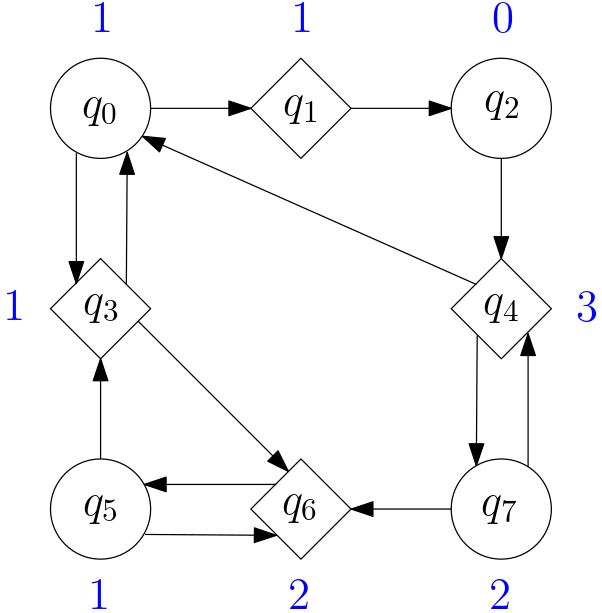
\includegraphics[width=0.4\textwidth]{figures/parity_game}
	\caption{An example of an arena. Circles  belong to player $0$, whereas diamonds belong to player $1$. Arrows represent transitions from a configuration to the next. The priority assigned by the priority mapping to each configuration is a number in $\{0,1,2,3\}$, next to the configuration it is assigned to. Note that we do not have a dead end in our example.}
	\label{example_parity_game}
	\end{figure}
\end{center}

\begin{example}
Let us consider the arena presented in  Figure~\ref{example_parity_game}. 
Configurations are partitioned into two sets: the circles, belonging to player $0$, and the diamonds,
belonging to player $1$. 
The priorities are $\{ 0,1,2,3\}$.
% The transitions and priority mappings may be derived from the picture.
% Note that we don't have a dead end in our example. 
Consider the game on the arena, where the winning condition is a parity condition.
Plays $\pi_1 = q_0 q_1 q_2 (q_4 q_7)^\omega$ and 
$\pi_2 = (q_0 q_1 q_2 q_4)^\omega$ are both winning for player $0$. Indeed, in $\pi_1$, 
the minimal priority encountered infinitely often is %that of $q_7$, that is, 
				$2$, 
whereas in $\pi_2$, it is %that of $q_2$, that is, 
			$0$. 
In both cases, it is an even number. On the other hand,
the plays $\pi_3 = (q_5 q_3 q_6)^\omega$ and $\pi_4=(q_5 q_6)^\omega$ are both winning for player $1$: the minimal priority encountered is odd, since it is $1$ for both.

One can take matters further: on this arena, player $0$ has a winning strategy for the parity game from $q_0$, $q_1$, $q_2$, $q_4$ and $q_7$, but not from $q_5$, $q_3$ nor $q_6$, where player $1$ has a winning strategy. 
\end{example}



One important property of parity games is that of {\em memoryless determinacy}: for a parity game
$\mathcal{G}= ((S_0,S_1,\rightarrow),\win_\Omega) $ and an initial configuration $s \in S_0 \cup S_1$, one of the players has a memoryless winning strategy from $s$ \cite{zielonka1998infinite}.

%\mh{
Of note is that several model checking problems %for pushdown automata 
can be expressed as decision problems for games: the most famous example is that the modal $\mu$-calculus model checking problem is polynomially equivalent to solving the parity game problem. 
%}


\section{Parametric pushdown games}





\textcolor{black}{Parametric pushdown automata extend pushdown automata by allowing the stack to be compared against parameters that can be assigned values which are words over the stack alphabet.}
A parametric pushdown automaton is then a finite automaton extended with a finite set of parameters $P$  and with a stack that can be manipulated by pushing or popping stack symbols and such that, moreover, the automaton can use the top of the stack, or check that the stack content corresponds to a parameter,  to decide which transition to take next.\\

\par\noindent\ignorespacesafterend
A {\em parametric pushdown automaton} ({\em PPDA} for short) 
is a tuple $\mathcal{Z} = (Q, \Gamma, P, R, q_{init},\gamma_{init}, F),$ where
 $Q$ is a non-empty finite {\em set of  states};
 $\Gamma$ is a non-empty finite {\em  stack alphabet};
 $P$ is a finite {\em   set of parameters}, \textcolor{black}{with $\Gamma \cap P = \emptyset$};
% \item  $R   \subseteq  Q  \times (\Gamma \biguplus P)  \times Q  \times \Gamma^*$ is finite {\em  set of rules},
  $R   \subseteq  Q  \times (\Gamma \biguplus P)  \times Q  \times \Op(\Gamma)$ is finite {\em  set of rules};
 $q_{init}\in Q$ is an {\em initial  state};
 $ \gamma_{init} \in \Gamma$ is an {\em initial stack symbol}; and
 $F\subseteq Q$ is a {\em set of final  states}.


The {\em size} of $\mathcal{Z}$ is defined as
$|\mathcal{Z}| = |Q| + |\Gamma| + |P| + |R| $.
We also refer to $\mathcal{Z}$ as an $n$-parametric pushdown automaton if $|P| = n$.
A {\em stack content} is a word from $ \Gamma^*$. 
As before we write the top
of the stack at the right of the word%(we are considering suffix rewriting as in Chapter 15)
. 
% A configuration is a  state and a stack content: $(q, w)$,
% which we rather write $q(w)$, where $w  \in  W^*$, $q  \in Q$. 
By $\Conf(\mathcal{Z})=Q\times  \Gamma^*$ we denote the set of
{\em configurations} of $\mathcal{Z}$. As usual we rather write $q(w)$ instead of $(q, w)$.
A {\em parameter valuation} is a function $\mu$ from $P$ to $\Gamma^*$.

\begin{samepage}
%\begin{definition}
A parametric pushdown automaton  $\mathcal{Z}= (Q, \Gamma, P,u R, q_{init}, \gamma_{init},F)$ 
and a parameter valuation $\mu: P\rightarrow \Gamma^*$ induce the 
%labeled 
transition system  
$T_{\mathcal{Z}}^{\mu} = (\Conf(\mathcal{Z}), 
%\Lambda_{\mathcal{Z}}, 
\rightarrow_{\mathcal{Z},\mu})$ where
% $\Lambda_{\mathcal{Z}} = \Gamma \cup P$ and
for all $ q, q'  \in  Q$, 
for all $ w,w' \in \Gamma^* $, and 
for all $ a  \in  \Gamma$, 
\iffalse
\begin{eqnarray*}
q(wa) \xrightarrow{%a
}_{\mathcal{Z},\mu} q'(w') & \text{if} &  (q, a, q' , op)  \in  R, \\
q(\mu(p) ) \xrightarrow{%p
}_{\mathcal{Z},\mu} q'(\mu(p) %\textcolor{red}{\cdot} 
w) & \text{if} &  (q, p , q' , w)  \in  R.
\end{eqnarray*}
% \end{definition}
\fi
$q(wa) \xrightarrow{%a
}_{\mathcal{Z},\mu} q'(w')$
if there exists a rule in $R$
 of the form $(q,a,q', op)$ or $(q,p,q', op)$ with $\mu(p)=wa$,
such that
		% $\text{\textit{top}}(w) = a$
		% and 
% $w' = \theta(w)$.
either of the following holds
\begin{itemize}
\item $ op = \text{\textit{push}}^\gamma$ and $w' = wa\gamma$,

\item $ op = \text{\textit{pop}}$ and $w' = w$, or

\item $ op = \text{\textit{skip}}$ and $w' = wa$.
\end{itemize}
\end{samepage}


A {\em $\mu$-run} from $q_0(a_0)$ to $q_n(a_n)$ in $\mathcal{Z}$ is a corresponding
path in the transition system 
$T_{\mathcal{Z}}^\mu$ 
induced by $\mathcal{Z}$ and $\mu$.
%
%and will be noted
%$q_0(z_0) \xrightarrow{\lambda_0}_{\mathcal{Z},\mu} q_1(z_1) \xrightarrow{\lambda_1}_{\mathcal{Z},\mu} \cdots \xrightarrow{\lambda_{n-1}}_{\mathcal{Z},\mu} q_n(z_n)$.
%
As with PDA, we say $\pi$ is {\em accepting} if $q_0 = q_{init}$, $a_0=\gamma_{init}$,
and $q_n\in F$.
%
% We say {\em reachability holds} for $\mathcal{Z}$ if there is a $\mu$ such that there is a $\mu$-run in $\mathcal{Z}$ from $q_{init}(\gamma_{init})$   to some configuration $q(w)$ for some $q\in F$ and some $w \in \Gamma^*$.
% We refer to Figure~\ref{example_pda} for an instance of a PDA for which reachability holds.




In the particular case where $P=\{p\}$ is a singleton for some parameter $p$ and $\mu(p)=u \in \Gamma^*$,
we prefer to write $q(w)\xrightarrow{%\lambda
}_{\mathcal{Z}, u}q'(w')$
to denote $q(w)\xrightarrow{%\lambda
}_{\mathcal{Z}, \mu}q'(w')$ and
will call the $\mu$-run an {\em $u$-run}. In case the automaton $\mathcal{Z}$ is obvious from context, we write $\xrightarrow{%\lambda
}_{\mu}$ (resp. $\xrightarrow{%\lambda
}_{u}$)
instead of $\xrightarrow{%\lambda
}_{\mathcal{Z}, \mu}$ (resp. $\xrightarrow{%\lambda
}_{\mathcal{Z},u}$). \\


		\iffalse	

\subsection{PPDA reachability}

Note that the reachability problem for parametric pushdown automata consists in
the following decision problem.

\problemx{$n$-PPDA reachability}
{An $n$-PPDA $\mathcal{Z}$.}
{Does 
%reachability hold for
an accepting $\mu$-run for some $\mu\in(\Gamma^*)^P$ exist in
 $\mathcal{Z}$?\newline}

		\fi

% \subsubsection{Parametric pshdown games}
\subsection{PPDA games}


Several model checking problems can be
expressed as decision problems for games.
For instance 
in the case of pushdown automata, 
the modal $\mu$-calculus
model checking problem is polynomially equivalent to solving the parity game problem.
% \textcolor{red}{Since the model checking problem has a more varied range of applications than the reachability problem (mb have a source for that or smtg)},
Since we are interested in parametric model checking and specification,
we are naturally interested in parametric variants of reachability games and parity games.

One goal may be to characterize the set of all possible parameter valuations for which a player has a winning strategy in a 
reachability game or a parity game
played on the arena induced by the
resulting concrete automaton
and some partition of its set of states. 
For determining such a set of parameter valuations, we incorporate the choice of the parameter valuation to the game. Each player then wants the parameter valuation to lead to an arena where it has a winning strategy.

In keeping with the spirit of alternation between players choosing successors in the arena, we consider here games where players
alternate choosing values for the parameters before alternating choosing successor configurations in the game on the induced arena.
For simplicity's sake, the values are assigned to the parameters one by one, alternating between values assigned by player $0$ and by player $1$.

A winning strategy for player $0$ allows to synthesize a controller that restricts the environment and ensures that {the property expressed by the winning condition always holds.}

% \subsection{Parameter valuation arenas}

We introduce here arenas over the set of partial parameter valuations for a set of parameters
$P = P_0 \biguplus P_1$. The values are assigned to the parameters one by one, alternating between values assigned by player $0$ (corresponding to parameters in $P_0$) and by player $1$ (corresponding to parameters in $P_1$). Other options could have been considered: for instance, we could consider a fully existential approach 
(i.e. all parameters have their values assigned by player $0$), 
or a fully universal approach
(i.e. all parameters have their values assigned by player $1$). 
Note however that the approach considered here encompasses both of the latter approaches:
the fully existential approach consists in the case where $P_1 = \emptyset$ and
the fully universal one, the case $P_0 = \emptyset$.



Assume an ordering of the parameters $P_0 \biguplus P_1 = \{p_0, p_1, \ldots, p_k \}$ for some 
%\textcolor{red}{even}
 $k \in \N$.
%
Then given a alphabet $\Gamma$, a {\em parameter valuation arena} is a tuple $A_{P_0,P_1,\Gamma} = (S_0, S_1, \rightarrow_P)$ where
\begin{itemize}

\item $S_0$ is the set of all partial parameter valuations with images in $\Gamma^*$ and domain $\{p_0, p_1, \ldots, p_{j}\} \setminus \{p_j\}$ where $\p_j \in P_0$,

\item $S_1$ is the set of all partial $\M$-parameter valuations  with images in $\Gamma^*$ and  domain $\{p_0, p_1, \ldots, p_{j}\} \setminus \{p_j\}$ where $\p_j \in P_1$,

\item
$ \mu \rightarrow_P \mu'$,
if $\mu' \in (\Gamma^*)^{\{p_0, \ldots, p_j\}}$ for some $j \in [0,k]$,
$\text{Dom}(\mu) = \text{Dom}(\mu') \setminus \{p_j\}$
and
 $\mu'(p) = \mu(p)$ for $p \in \text{Dom}(\mu)$. \label{parametric arena}
\end{itemize}


Note that the arena has dead ends, and that these are the configurations that correspond to parameter valuations.
Given a strategy $\sigma_0$ for player $0$ and a strategy $\sigma_1 $ for player $1$,
the last configuration of the resulting play $\pi(\mu_\bot,\sigma_0, \sigma_1)$
is called {\em the resulting parameter valuation}
 and is denoted by $\mu_{\sigma_0, \sigma_1}$, where 
 $\mu_\bot$ is the partial parameter valuation with domain $\emptyset$. 
 %We do not really consider winning conditions for parameter valuation games. Rather, once the resulting parameter valuation is produced, it serves to instantiate the parametric transition system for the next game.
Parametric valuation arenas can then be used as prefixes in parametric games. Once the resulting parameter valuation is produced by the two players, it serves to instantiate the transition system for continuing the game.
%
%
Indeed, where a concrete automaton induces a transition system, a parametric automaton induces one transition system for every possible parameter valuation.
We use $T^\mu_\A$ to denote the transition system induced by the concrete automaton corresponding to
a parametric automaton $\A$ with parameters $P$ taking values in $\Gamma^*$ and a parameter valuation $\mu: P \to \Gamma^*$.


\iffalse
\begin{center}
	\begin{figure}
		\hspace{2cm}
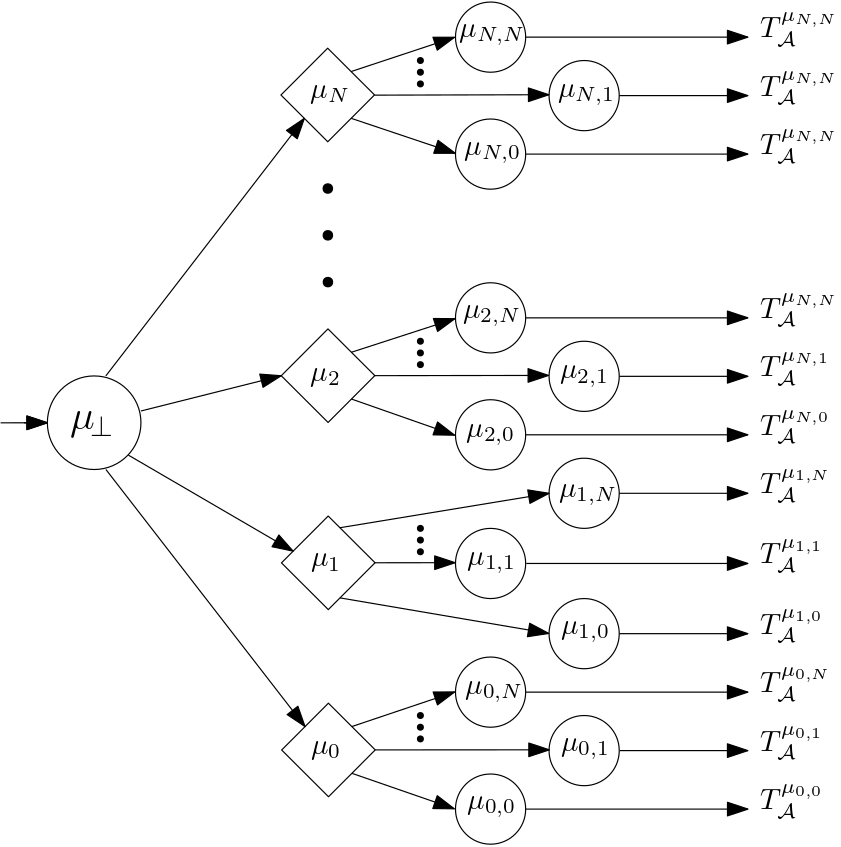
\includegraphics[width=0.7\textwidth]{figures/parameter_arena}
	\caption{An illustration of the arena for a parametric automaton $\A$ with 
%	two parameters, $p_0$ and $p_1$,	
	$P_0 = \{p_0\}$, $P_1 = \{p_1\}$ and
%	 that can take values in $[0,N]$ for some $N \in \N$. 
	$\M = [0,N]$ for some $N\in \N$.
	 Here $\mu_\bot$ is 
	%the partial parameter assignment with domain $\emptyset$,
	the totally undefined function and can be viewed rather as 
	the function that assigns $\bot$ to both parameters. For $i,j \in [0,N]$, $\mu_i$ is the partial parameter assignment with domain $\{p_0\}$ that maps $p_0$ to $i$ and $\mu_{i,j}$ is the parameter assignment that maps $p_0$ to $i$ and $p_1$ to $j$.
	 %Lastly $T^\mu_\A$ denotes the transition system induced by the concrete automaton corresponding to $\A$ with parameter valuation $\mu$.
	  As before, the circles belong to player $0$ and the diamonds to player $1$.} 
	\label{parametric_arena}
	\end{figure}
\end{center}
\fi


\iffalse
Given a parametric automaton $\A$ with a set of parameters $P = P_0 \biguplus P_1$ that can take 
values in the set $\Gamma^*$,
a {\em parametric game} for $\A$ is a game played 
on the 
arena $A_\A$
that include both 
the parameter valuation arena
$A_{P_0, P_1,\Gamma}$
and, %   
for all parameter valuations $\mu: P\rightarrow \Gamma^*$,
the transition system %s 
 $T_\A^\mu$
\---- albeit with configurations additionally indexed by $\mu$ %in the tuple
 to avoid confusion.
Moreover, for every 
dead end $\mu$
 in $A_{P_0,P_1,\Gamma}$,
we add a transition
from the configuration $\mu \in (\Gamma^*)^P$ to
$T_\A^\mu$.
% See Figure~\ref{parametric_arena} for an illustration of such an arena.
\fi
 
Recall that given a 
%labeled 
transition system,
one needs only to provide %a mapping $\Omega$ and 
a partition of the set of configuration $S$ into two sets $S_0$ and $S_1$ to obtain an arena. 
Thus, for an  $n$-parametric pushdown automaton 
$\mathcal{Z}= (Q, \Gamma, P, R, q_{init}, \gamma_{init},F)$,
given a partition of
$Q$ into $Q_0$ and $Q_1$, 
we naturally partition the configurations of
%the transition system of 
 $\mathcal{Z}$
% $T^\mu_{\mathcal{Z}}$
into
$\Conf_{\mathcal{Z},0}=Q_0\times \Gamma^*$
and
$\Conf_{\mathcal{Z},1}=Q_1\times \Gamma^*$. 


With these notations in mind one can define the arena
\[
A_{(\mathcal{Z}, Q_0, Q_1, \mu)}
=
(\Conf_{\mathcal{Z},0}, \Conf_{\mathcal{Z},1}, \rightarrow_{\mathcal{Z},\mu})\]
induced by a PPDA $\mathcal{Z}$, a partition of its set of states, and a
parameter valuation $\mu: P\rightarrow \Gamma^*$.



From a partition of
$P$ into $P_0$ and $P_1$, 
we thus define 
$A_{(\mathcal{Z}, P_0, P_1, Q_0 , Q_1)}$
as
the arena that contains both the configurations and transitions of
the parameter valuation arena
$A_{P_0,P_1,\Gamma}$,
and that moreover contains the configurations and transitions of
$A_{(\mathcal{Z}, P_0, P_1, Q_0 , Q_1, \mu)}$ 
\---- albeit with configurations additionally including $\mu$ in the tuple to avoid confusion \----
for
all parameter valuations $\mu: P\rightarrow \Gamma^*$.
Moreover, for every configuration $\mu$ in $A_{P_0,P_1,\Gamma^*}$,
we add a transition
from $\mu$ towards 
$q_{init}(\gamma_{init}, \mu)$ in $A_{(\mathcal{Z}, P_0, P_1, Q_0 , Q_1, \mu)}$. \label{PPDA reachability game}




Given a 
priority function $\Omega: Q \to [0, m]$,
we consider the function
$\widehat{\Omega}: \Conf(\mathcal{Z}) \cup (\Gamma^* \cup \bot)^{[0,n]} \to [0, m]$
where we set
$\widehat{\Omega}(q, w, \mu) = \Omega(q)$
for all
$w \in \Gamma^*$
and
for all $\mu \in (\Gamma^*)^{P}$,
and
$\widehat{\Omega}(\mu) = 0$
for all $\mu \in (\Gamma^* \cup \bot)^{P}$.



\problemx{Parametric pushdown reachability game}
{A parametric pushdown automaton $\mathcal{Z}= (Q, \Gamma, \{p_0, p_1, \ldots, p_k \}, R, q_{init},  \gamma_{init} , F)$, where $Q = Q_0  \biguplus Q_1 $%which naturally lead to a partition of $T_{\mathcal{Z}}$
, and $ P = P_0 \biguplus P_1$.}
{Does player $0$ have a winning strategy from $\mu_\bot$ in the reachability game \\
$\mathcal{G} =(A_{(\mathcal{Z}, P_0, P_1, Q_0 , Q_1)}, \win_{F \times \Gamma^* \times (\Gamma^*)^P})$ ?\newline}




\problemx{Parametric pushdown parity game}
{A parametric pushdown automaton $\mathcal{Z}= (Q, \Gamma, \{p_0, p_1, \ldots, p_k \}, R, q_{init}, \gamma_{init} , F)$, where $Q = Q_0  \biguplus Q_1 $%which naturally lead to a partition of $T_{\mathcal{Z}}$
, and $ P = P_0 \biguplus P_1$, 
and a priority function $\Omega: Q \to [0, m]$%
%which naturally lead to a mapping on $\Conf(\mathcal{Z})$
%, and an initial state $q_{init} \in Q$% and initial stack symbol $w_{init} \in W$
.}
{Does player $0$ have a winning strategy from $\mu_\bot$ in the parity game \\
$\mathcal{G} =(A_{(\mathcal{Z}, P_0, P_1, Q_0 , Q_1)}, \win_{\widehat{\Omega}})$ ?\newline}





We write {\sc $n$-parametric reachability parity game}
and
{\sc $n$-parametric pushdown parity game} if 
 the number of parameters $n=|P|$ of $\mathcal{Z}$ is fixed by the problem.
Remark that the parametric reachability problem for an automaton with parameters can be seen as solving the parametric reachability game where $P_1 = \emptyset$, and $Q_1 = \emptyset$.
We are interested in the following games and problems.



			
			
				
				
				


%\subsection{A decidability result from reduction to parity games on automata with pebbles}\label{pebbles}
\section{%A decidability result via r
Reduction to pebble pushdown automata parity games
}\label{pebbles}



% \mh{Motivates the use of pebbles. See pebbles on two-way automata, two-way tree automata, weighted automata, etc.}



% 21. Globerman, N., Harel, D.: Complexity results for two-way and multi-pebble automata and their logics. Theor. Comput. Sci. 169, 161–184 (1996)
%		same as [13] bellow
%
% Engelfriet, J., Hoogeboom, H.J.: Tree-walking pebble automata. In: Karhumäki, J., Maurer, H., Pa ̆un, G., Rozenberg, G. (Eds.) Jewels are Forever, Contributions to Theoretical Computer Science in Honor of Arto Salomaa, pp. 72–83. Springer, Berlin (1999) for tree-walking automata.
%
% @incollection{engelfriet1999tree,
%  title={Tree-walking pebble automata},
%  author={Engelfriet, Joost and Hoogeboom, Hendrik Jan},
%  booktitle={Jewels are forever},
%  pages={72--83},
%  year={1999},
%  publisher={Springer}
%}
% 
%
% Two-way pebble transducers for partial functions and their composition, Joost Engelfriet
%
% Tree-Walking Pebble automata, Joost Engelfriet and Hendrik Jan Hoogeboom 
A pebble automaton is a two-way finite state automaton that uses a fixed, finite number of
pebbles that it can drop on, and lift from 
words, using them as markers.
Pebble automata recognize regular languages only, provided the life times of the pebbles, i.e. the times between dropping a pebble and lifting it again, are properly nested
\cite{globerman1996complexity, engelfriet1999tree}.
Automata with nested pebbles were also introduced
for tree-walking automata. 
It is known that tree-walking automata do not recognize all regular tree languages \cite{bojanczyk2008tree}%, the main trouble being that tree-walking automata get lost rather easily
.
Using pebbles is a remedy against getting lost along a tree, but 
the unrestricted use of pebbles leads to a class of tree languages much larger than the
regular tree languages, in fact to all tree languages in $\NSPACE(log ~ n)$.
Thus, in  both pebble word automata and pebble tree-walking automata, the placement of the pebble follows a strict stack discipline. It is traditional hence to represent syntactically the dropping and lifting of pebbles by operations \textit{lift} and \textit{drop}; a \textit{drop} simply records the current position with a fresh pebble (such a pebble should be available) % and returns to the beginning of the tape, 
and a \textit{lift} pops the last dropped pebble if the current position corresponds to the one recorded by it.




In this section, we extend these ideas to pushdown automata. Instead of using pebbles as markings on their input, pebble pushdown automata have the ability to lift or drop pebbles on their universe of stack contents; a \textit{drop} simply records the current stack content with a fresh pebble (such a pebble should be available) % and returns to the beginning of the tape, 
and a \textit{lift} pops the last dropped pebble 
while requiring that
% assuming
 it was placed on the current node. 
% Thus hierarchicality on the registers works slightly differently from hierarchicality on the pebbles, hierarchicality on the registers being a syntactic property, whereas hierarchicality on the pebbles is a semantical one.
One can think of a pebble as a register that can store a stack content for later comparisons.



We first define more formally our pebble pushdown automaton framework, and then provide a reduction from the problem of solving parametric pushdown parity games to the problem of solving pebble pushdown parity games.



%\subsubsection{Pebble pushdown automata}
\subsection{Pebble pushdown automata}

\newcommand{\ppda}{\mathcal{I}}
% \Denarius
% \vernal
% \mathscr{Z}
% \mathcal{I}
% \pluto
% \capricornus
% \Bumpeq
% \Pfund

An {\em $n$-pebble pushdown automaton} 
is a tuple 
$\ppda = (Q, \Gamma,  R, q_{init}, \gamma_{init}, F)$
where $Q$ is a {\em finite set of  states}; $\Gamma$ is a {\em finite stack alphabet};
  $R  \subseteq  Q  \times \Gamma \times
		 \{ 0, 1, \ldots n\} \times \mathcal{P}(\{1,\ldots,n\})
		 \times Q  \times (\Op(\Gamma) \cup \{\text{\textit{drop}}, \text{\textit{lift}}\})$ is a {\em finite set of rules},
		 where the fourth element $S$ of a rule $r$ is a subset of 
		$\mathcal{P}(\{1,\ldots,i\})$ where $i$ is the third element of $r$,
		and if the last element is
		$\text{\textit{lift}}$ then we additionally require $i \in S$;
 $q_{init} \in Q$ is an {\em initial  state};
 $\gamma_{init} \in \Gamma$ is an {\em initial stack symbol}; and
 $F \subseteq Q$ is a {\em set of final  states}.


 
%%%%%%%%%%%%%%%%%%%%%%%%%%%%%%%%%%%%%%%%%%%%%%%%%%%%%%%%%%% 
% \mh{remind the reader what a partial function is}
 
\par\noindent\ignorespacesafterend 
Recall that for a partial function $ f : S \rightharpoonup X $% (see page~\pageref{partial})
, for notational purposes, we consider some element $\bot_X \not\in X$ and 
 associate $f$ with the function returning the 
bottom element $\bot_X$ when $f$ is undefined. Thus we write $(X \biguplus \{ \bot_X \})^S$ for the set of all partial functions from $S$ to $X$, which we here abbreviate as $(X \biguplus \{ \bot \})^S$. 


%%%%%%%%%%%%%%%%%%%%%%%%%%%%%%%%%%%%%%%%%%%%%%%%%%%%%%%%%%%
 
 
% An $i$-configuration of $\ppda$ is an element of
%$ Q\times W^* \times (W^*)^{\{1, \ldots i\}}$.
% By $\Conf_i(\ppda)$ we denote the set of $i$-configurations of $\ppda$.
By $\Conf(\ppda)=Q\times \Gamma^* \times (\Gamma^* \biguplus \{ \bot \})^{\{1, \ldots, n\}}$ we denote the set of
% By $\Conf(\ppda) = \bigcup_{0 \leq i \leq n} \Conf_i(\ppda)$ we denote the set of
{\em configurations} of $\ppda$. As expected, we rather write $q(w, \mu)$ instead of $(q, w, \mu)$.
An {\em$i$-configuration} for $i > 0$ of $\ppda$ is a configuration $q(z,\mu)$ where
$\text{Dom}(\mu) = \{1, \ldots, i\}$, while a $0$-configuration is a configuration 
 $q(z,\mu)$ where $\text{Dom}(\mu)=\emptyset$.



The idea of a transition $(q, a, i, S, q', m) \in R$
is that, if the automaton $\ppda$ is in state $q$ with pebbles $1,\ldots, i$ dropped \---- or without pebble dropped if $i = 0$ \---- with top stack symbol $a$, and stack content which corresponds to the stack contents of the pebbles from $S$ and only these pebbles, then
$\ppda$ goes to state 
$q'$ and makes modifications to the stack or the pebbles according to
$m$. 
% \mh{The set $S$ is used for testing the presence of certain pebbles.}
Note a pebble 
can be lifted only if the stack content which corresponds to the pebble
is the same as the current stack content. 
%$\Dzeta$ $\zeta$ $\Xi$
This is enforced by syntactically requiring
the last pebble dropped $i$ is in the set $S$ used for testing the presence of certain pebbles.

\iffalse
A {\em weak} $n$-pebble pushdown system is an $n$-pebble pushdown system $\ppda = (Q, \Gamma,  \Delta )$ in which $\text{\textit{lift}}$ operations also require the presence of the last pebble dropped, i.e.
for all $(q, a, i, S, q', \text{\textit{lift}}) \in \Delta$, we have $ i \in S $. 
%  is an additionnal restriction $f(i) = wa$ that needs to hold for the application of the $lift$ operation.
{\em Weak $n$-pebble pushdown games} are defined naturally as $n$-pebble pushdown games on 
weak $n$-pebble pushdown systems.

\fi



A {\em pebble set} of $\ppda$ is a set $U \subseteq \{ 1, \ldots, n\}$. For a stack alphabet $\Gamma$, a 
{\em $U \!$-pebble assignment} is a function which maps each $j \in U$ to a word in $ \Gamma^*$.
The $\emptyset$-pebble assignment is denoted by $\mu_{init} :  \{ 1, \ldots, n\} \rightharpoonup  \Gamma^* $ and is the 
%partial function from  $\{ 1, \ldots, n\}$ to $ \Gamma^* $ that
%does not map any $j \in \{ 1, \ldots, n \}$ to an output.
totally undefined function.


\iffalse
For $0 \leq i \leq n$, an {\em $i$-configuration} is a tuple $(q, w, \mu )$, where $w \in \Gamma^*$, $q$ is a state and
$\mu$ a $\{ 1, \ldots , i \}$-pebble assignment. 
We call $w$ the current stack, $q$ the current state and
$\mu$ the current pebble assignment. 
We also write $(q,w, w_{1} , \ldots , w_{i} )$ if 
$\mu(j) = w_j$, for each
$j \leq i$.

The set of configurations is the union of all $i$-configurations for $0 \leq i \leq n$. 
\fi


\begin{samepage}
%\begin{definition}
An $n$-pebble pushdown automaton $\ppda =  (Q, \Gamma,  R, q_{init}, {\gamma_{init}} , F)$ induces 
a transition system  $T_{\ppda} = (\Conf(\ppda), \rightarrow_{\ppda})$ 
 such that
for all $(q, a, i, S, q', m) \in R$, with $a \in \Gamma$,
 for all words $w \in  \Gamma^*$, and for all $\{ 1, \ldots , i \}$-pebble assignments $\mu$ such that $\mu(j) = wa$ 
 %(respectively $\mu(j)= {\gamma_{init}}  $) 
 for each
$j \in S$ 	and
 $\mu(j) \neq wa$ 
 %(resp. $\mu(j) \neq {\gamma_{init}} $) 
 for each $j \in \{ 1, \ldots , i \} \setminus S$,
the following holds
\begin{itemize}
\item if $m \in \Op(\Gamma)$, 
% $(q,wa,\mu) \rightarrow_{\ppda} (q',wm, \mu)$, 
either
\begin{itemize}
\item $ m = \text{\textit{push}}^\gamma$ and $(q,wa,\mu) \rightarrow_{\ppda} (q',wa\gamma, \mu)$,

\item $ m = \text{\textit{pop}}$ and $(q,wa,\mu) \rightarrow_{\ppda} (q',w, \mu)$, or

\item $ m = \text{\textit{skip}}$ and $(q,wa,\mu) \rightarrow_{\ppda} (q',wa, \mu)$,
\end{itemize}
\item if $ m = \text{\textit{drop}}$, 
$(q,wa,\mu) \rightarrow_{\ppda} (q',wa, \mu')$,  
where $\mu'$ is the $\{ 1, \ldots , i, i+1 \}$-pebble assignment such that
$\mu'(j) = \mu(j)$, for each
$j \leq i$, and $\mu'(i+1) = wa$, and
\item if $m = \text{\textit{lift}}$, and $i \in S$, i.e. the last pebble dropped belong of the set of pebble we test the presence of,
$(q,wa,\mu) \rightarrow_{\ppda} (q',wa, \mu')$, 
where $\mu'$ is the $\{ 1, \ldots , i - 1 \}$-pebble assignment such that
$\mu'(j) = \mu(j)$, for each
$j < i$.
\end{itemize}
%\end{definition}
\end{samepage}


\par\noindent\ignorespacesafterend
We are interested in games over pebble pushdown automata, % namely, 
%reachability, B\"uchi, and parity games.
mainly, parity games.

Again, given
a 
%labeled
 transition system, one needs only to provide 
%a mapping $\Omega$ and 
a partition of the set of
configurations 
%$S$ into two sets $S_0$ and $S_1$
 to obtain an arena.
 %
Given a partition of
$Q$ into $Q_0$ and $Q_1$, 
we partition the configurations of
$T_{\ppda}$
into
$\Conf_{\ppda,0}=Q_0\times \Gamma^* \times ( \Gamma^* \biguplus \{ \bot \})^{\{1, \ldots n\}}$
and
$\Conf_{\ppda,1}=Q_1\times  \Gamma^* \times ( \Gamma^* \biguplus \{ \bot \})^{\{1, \ldots n\}}$. 



With these notations in mind one can  define the arena
$$
A_{(\ppda, Q_0 , Q_1)}
=
(\Conf_{\ppda,0}, \Conf_{\ppda,1}, \rightarrow_{\ppda}).$$




As expected, given a 
priority function $\Omega: Q \to \{0, \ldots m\}$,
one naturally 
set the extension of $\Omega$ as
$\overline{\Omega}: \Conf(\ppda) \to \{0, \ldots m\}$
and
$\overline{\Omega}(q, w,\mu) = \Omega(q)$
for all
$w \in  \Gamma^*$
and
$\mu \in ( \Gamma^* \biguplus \{ \bot \})^{\{1, \ldots, n\}}$. \\









Concerning pebble pushdown automata, we are interested in the following decision problem.


\problemx{$n$-pebble pushdown parity game}
{An $n$-pebble pushdown automaton $\ppda= (Q, \Gamma,  R, q_{init}, {\gamma_{init}} , F)$, 
where $Q = Q_0  \biguplus Q_1 $, 
and
a priority mapping $\Omega: Q \to \{0, \ldots m\}$.}
{Does player $0$ have a winning strategy from $q_{init}(\gamma_{init}, \mu_{init})$ for the parity game 
$\mathcal{G}= (A_{(\ppda, Q_0 , Q_1)}, \win_{\overline{\Omega}})$ ?\newline}



% \subsubsection{Reduction from parameters to pebble pushdown automata}
\subsection{From parametric pushdown 
automata 
to pebble pushdown automata
}

We now provide a reduction from the problem of solving parametric pushdown parity games to the problem of solving pebble pushdown parity games. 


\begin{theorem}\label{PPDA reduction}
%The problem of 
{\sc $n$-parametric pushdown parity game} 
is polynomial time reducible to
%the problem of 
{\sc $n$-pebble pushdown parity game}.
\end{theorem}




\begin{proof}[Sketch]


Let us fix some
$n$-parametric pushdown automaton $\mathcal{Z}= (Q, \Gamma, 
P%\{p_1, \ldots, p_n \}
, q_{init}, { \gamma_{init}} , F)$,
 disjoint
union $Q = Q_0  \biguplus Q_1$
and $P = P_0 \biguplus P_1$,
and
some priority function 
$\Omega : Q \times \Gamma^* \times ( \Gamma^* \biguplus \{ \bot \})^R \to [0, m ]$.


We construct
% polynomial time
  an 
 $n$-pebble pushdown automaton $\ppda =(Q', \Gamma,  R', q_{init}', {\gamma_{init}} , F')$,
a 
 disjoint
union $Q' = Q_0'  \biguplus Q_1'$
and a mapping $\Omega' : Q \times  \Gamma'^* \times ( \Gamma'^* \biguplus \{ \bot \})^{\{1, \ldots, n\}} \to \{1, \ldots, m \}$,
such that
 %:
%
player $0$ has a winning strategy from 
$(q'_{init},\gamma_{init}, \mu_{init})$
in
		\iffalse
		for the parity condition on
		$\mathcal{G}_{(\ppda, Q'_0, Q'_1, \Omega')}$.
		\fi
the parity game
$\mathcal{G'}= (A_{(\ppda, Q'_0, Q'_1)}, \win_{\overline{\Omega'}})$
if and only if
player $0$ has a 
		\iffalse
		strategy $\sigma_0$ for the parameter valuation game  such that
		for all player $1$ strategies $\sigma_1$ for the parameter valuation game,
		player $0$ have a
		winning strategy from $q_{init}(\gamma_{init})$ for the parity condition on
		$\mathcal{G}_{(\mathcal{Z}, \mu_{\sigma_0, \sigma_1}, P_0, P_1, Q_0 , Q_1, \Omega)}$. 
		\fi
winning strategy from $\mu_\bot$ in 
the parity game
$\mathcal{G} =(A_{(\mathcal{Z}, P_0, P_1, Q_0 , Q_1)}, \win_{\widehat{\Omega}})$,
where		 
$A_{(\mathcal{Z}, P_0, P_1, Q_0 , Q_1)}$
and
$\widehat{\Omega}$
correspond to the definitions on page~\pageref{PPDA reachability game}.

%
%
%
%


The transition graph of the $n$-pebble pushdown automaton $\ppda$ will simulate the possible transitions graphs 
(one for every 
%total 
parameter assignment)
 of the pushdown automaton with $n$ parameters by using pebbles to represent the parameters. 
The $n$-pebble pushdown automaton will first simulate the 
parameter valuation arena.
Players take turns chosing particular stack contents on which to place pebbles. 
Once every parameter has been assigned with the dropping of a corresponding pebble, 
the pebble assignment $\mu$ is fixed.
%%
%
%
%
%
%
%


Further configurations in the $n$-pebble pushdown automaton then consist of a word representing the status of the stack, a state, and a fixed pebble assignment. For a fixed pebble assignment there is then a one for one correspondance between configurations of the $n$-parametric pushdown 
automaton 
%transition system with assignment $\mu$
and these of the $n$-pebble pushdown automaton. The set of states of the $n$-pebble pushdown automaton apart from the initial gadget is the same as 
the set of states of the $n$-parametric pushdown automaton, and 
so are player $0$ states, player $1$ states and the priority mapping.
\end{proof}




\section{Reduction to higher-order pushdown automata}\label{section HPDA}




Higher-order pushdown automata (HPDA for short) were introduced as a 
generalization of pushdown automata \cite{aho1969nested,Gre70,maslov1976multilevel}. 
% Alfred V. Aho. Nested stack automata. J. ACM, 16(3):383–406, 1969.
% S. Greibach. Full AFL’s and nested iterated substitution. Inf. Control, 16(1):7–35, 1970.
% A.N. Maslov. Multilevel stack automata. Problemy Peredachi Informatsii, 12:55–62, 1976.
A stack of a pushdown automaton is seen as a {\em level $1$ stack}. 
A pushdown automaton of level $2$ (or $2$-HPDA) then works with a stack of level $1$ stacks. 
In addition to the ability to push
and to pop a symbol on the top-most level $1$ stack, an $2$-HPDA can copy or remove the entire topmost level $1$ stack. 
The definition generalizes to any $n \geq 2$, and $n$-HPDA are similarly defined for all level
$n$ as automata working with a stack of level $(n-1)$ stacks.
% HPDA have been extensively studied as language recognizers [Dam82,Eng83].



We recall the definition from \cite{cachat2007complexity} which itself is taken from \cite{knapik2002higher}. We then provide a
reduction from the problem of solving pebble pushdown parity games to the problem of solving
higher-order pushdown parity games.


\subsection{Higher-order pushdown automata}

A {\em level $1$ stack} (or {\em $1$-stack}) over an alphabet $\Gamma$ is 
simply a %word in $\Gamma^*$
	stack over $\Gamma$, i.e. a word  in $\Gamma^*$.
% an arbitrary sequence $w_0 w_1 \ldots w_n $ of elements of $\Gamma$ for some $n \in \N$. 
A  {\em level $n$ stack} (or {\em $n$-stack}) over an alphabet $\Gamma$, for $n \geq 2$, is a 
non-empty sequence
$ \langle s_0 \rangle \langle s_1 \rangle \ldots \langle s_m \rangle$
of
$(n-1)$-stacks over $\Gamma$,
for some $m \in \N$.
The set of $n$-stacks over $\Gamma$ is denoted by $\mathscr{S}_n(\Gamma)$,
or simply $\mathscr{S}_n$ in case the set $\Gamma$ is obvious from context.
The set of all stacks over $\Gamma$ is written $\mathscr{S}(\Gamma) = \bigcup_{n\in \N} \mathscr{S}_n(\Gamma)$.
We define $\epsilon_{1}$ as
$\epsilon \in \Gamma^*$ and we inductively define 
$\epsilon_{n} = \langle \epsilon_{n-1} \rangle$ in $\mathscr{S}_n$ for all $n > 1$.




A {\em higher-order stack operation} is a partial function from $\mathscr{S}(\Gamma)$ 
to $\mathscr{S}(\Gamma)$ which preserves the level of the input (i.e. the image of
an $n$-stack is an $n$-stack for all $n \in \N$). The {\em level } of an operation $op$
is the smallest $n \in \N$ such that $\text{Dom}(op) \cap \mathscr{S}_n \neq \emptyset$. 
The operations 
%we consider
additionally
 respect the hierarchicality of higher-order stacks, i.e. in
a level $n+1$ stack only the topmost level $n$ stack can be accessed. An operation
$op$ of level $n$, applied to a level $n+1$ stack 
$ \langle s_0 \rangle \langle s_1 \rangle \ldots \langle s_m \rangle$
of length $m \in \N$,
thus
returns the output
$ \langle s_0 \rangle \langle s_1 \rangle \ldots \langle op(s_m) \rangle$
if applicable.
The definition for  all levels of stacks greater than $n$ follows the same pattern.


% For all $m \in \N$, 
The following operations can be performed on a $1$-stacks of length $m \in \N$.
% $ w_0 w_1 \ldots w_m \in \Gamma^*$.
\begin{eqnarray*}
&\text{\textit{push}}_1^\gamma( w_0 w_1 \ldots w_m) &=\quad w_0 w_1 \ldots w_m \gamma   \text{ for all } \gamma \in  \Gamma, \\
&\text{\textit{pop}}_1(w_0 w_1 \ldots w_{m-1} w_m ) &=\quad w_0 w_1 \ldots w_{m-1}, \text{ if } m \geq 1\\
&\text{\textit{top}}( w_0 w_1 \ldots w_m ) &=\quad w_m.
\end{eqnarray*}
The operations added at level $n+1$ are the copy of the topmost $n$-stack
and the removal of the topmost $n$-stack.
More formally, if $ \langle s_0 \rangle \langle s_1 \rangle \ldots \langle s_m \rangle$ is a stack of 
level $n > 1$, 
the following operations are possible.
%
\begin{eqnarray*}
&\text{\textit{push}}_n( \langle s_0 \rangle \langle s_1 \rangle \ldots \langle s_m \rangle) &=\quad  \langle s_0 \rangle \langle s_1 \rangle \ldots \langle s_m \rangle \langle s_m \rangle , \\
&\text{\textit{push}}_j( \langle s_0 \rangle \langle s_1 \rangle \ldots \langle s_m \rangle) &=\quad \langle s_0 \rangle, \langle s_1 \rangle \ldots 
\langle \text{\textit{push}}_j(s_m) \rangle,
\text{ if } 2 \leq j < n\\
&\text{\textit{push}}_1^\gamma( \langle s_0 \rangle \langle s_1 \rangle \ldots \langle s_m \rangle) &= \quad
\langle s_0 \rangle \langle s_1 \rangle \ldots 
\langle \text{\textit{push}}_1^\gamma(s_m) \rangle,
\text{ for all } \gamma \in \Gamma,\\
&\text{\textit{pop}}_n( \langle s_0 \rangle \langle s_1 \rangle \ldots \langle s_{m-1} \rangle \langle s_m \rangle) &= \quad
\langle s_0 \rangle \langle s_1 \rangle \ldots \langle s_{m-1} \rangle
,\\
&\text{\textit{pop}}_j( \langle s_0 \rangle \langle s_1 \rangle \ldots \langle s_{m-1} \rangle \langle s_m \rangle) &= \quad
\langle s_0 \rangle \langle s_1 \rangle \ldots \langle s_{m-1} \rangle
\langle \text{\textit{pop}}_j(s_m) \rangle,
\text{ if } 1 \leq j < n\\
&\text{\textit{top}}( \langle s_0 \rangle \langle s_1 \rangle \ldots \langle s_m \rangle) &=\quad
\text{\textit{top}}(s_m).
\end{eqnarray*}
% We omit the stack alphabet $\Gamma$ from 
%The operation $pop_j$ is undefined on a stack whose top stack of level $j$ is empty.
The operations $pop_1$ and $top$ are undefined on a stack whose top $1$-stack is empty.  \\


Given a stack alphabet $\Gamma$ and $n \in \N$, 
we denote by  $\Op_n(\Gamma)$ the {\em base set of $n$-stack operations} as

\begin{itemize}
\item $\text{\textit{push}}_j$ for all $2 \leq j \leq n$,

\item $\text{\textit{push}}_1^\gamma$ for all $\gamma \in \Gamma$,

\item $\text{\textit{pop}}_j$ for all $1 \leq j \leq n$,

\item $\text{\textit{skip}}$, corresponding to the identity function of $\mathscr{S}(\Gamma)$.

\end{itemize}




% \begin{definition}
\begin{samepage}
\par\noindent\ignorespacesafterend
A {\em higher-order pushdown automata of level $n$} (or $n$-HPDA for short) 
is a tuple $\H=(Q, \Gamma, R, q_{init}, \gamma_{init}, F)$,
where 
\begin{itemize}
        \item $Q$ is a non-empty finite {\em set of  states},
        \item $\Gamma$ is a non-empty finite {\em  stack alphabet},
	\item $R\subseteq Q\times \Gamma \times Q \times \Op_n(\Gamma)$ is a finite {\em set of  rules},
        \item $q_{init}$ is the {\em initial  state},
        \item $\gamma_{init} \in \Gamma$ is the {\em %bottom-of-stack
initial stack symbol}, and
	\item $F\subseteq Q$ is a {\em set of final  states}.
		\end{itemize}
\end{samepage}
% \end{definition}

\par\noindent\ignorespacesafterend
By $\Conf(\mathcal{H}) = Q \times \mathscr{S}_n(\Gamma)$
we denote the set of {\em configurations} of an $n$-HPDA $\H$. 
%is a pair $(q, s)$ where $q \in Q$ and $s$ is an $n$-stack over $\Gamma$. 
As usual we abbreviate $(q,s) \in \Conf(\mathcal{H})$ as $q(s)$.



An $n$-HPDA $\H=(Q, \Gamma, R, q_{init}, F)$
induces the transition system $\T_\H = (Conf(\mathcal{H}), \rightarrow_{\mathcal{H}})$
where
for all $q,q'$ in $Q$,
for all $s,s'$ in $\mathscr{S}_n(\Gamma)$,
$q(s) \rightarrow_{\mathcal{H}} q'(s')$ if
there exists some rule
%$(q,\gamma,q',\theta) \in R$
$(q,\gamma,q',op) \in R$
such that
$\text{\textit{top}}(s) = \gamma$
and
%$s' = \theta(s)$.
$s' = op(s)$.




\iffalse
For our constructions it would be simpler to assume that k-HPDS can work
also on stacks of lower levels, in particular on 1-stacks. Of course we can always
simulate a j-stack, for j < k with an k-stack but in the notation it requires some
additional parenthesis that make it less readable.

To define a game on the graph of a HPDA, we assign a player to each control
state, and we consider an initial configuration: a game structure on a HPDS H
is a tuple G = (H, P0 , P1 , s0 ), where P = P0 ⊎ P1 is a partition of the control
states of H, and s0 ∈ Sk . This extends naturally to a partition of the set of
configurations: with the notations of Section 2.1, V0 = P0 × Sk , V1 = P1 × Sk ,
and E is defined above.
\fi

Again we are interested in parity games.
As expected, given an 
 $n$-HPDA $\mathcal{H}$
 and a partition of
$Q$ into $Q_0$ and $Q_1$,
we partition the configurations of
$T_{\mathcal{H}}$
into
$\Conf_{\mathcal{H},0}=Q_0\times \mathscr{S}_n(\Gamma)$
and
$\Conf_{\mathcal{H},1}=Q_1\times\mathscr{S}_n(\Gamma)$.
%
%
With these notations in mind one can define the arena
$$
A_{(\mathcal{H}, Q_0, Q_1)}
=
(\Conf_{\mathcal{H},0}, \Conf_{\mathcal{H},1}, \rightarrow_{\mathcal{H}})$$
\par\noindent\ignorespacesafterend
induced by an $n$-HPDA $\mathcal{H}$ and a partition of its set of states.


As expected, given a 
priority function $\Omega: Q \to [0, m]$,
we naturally extend the function
as follows,
by setting
$\Omega_{\mathscr{S}_n(\Gamma)}: \Conf(\mathcal{H}) \to [0, m]$
and
$\Omega_{\mathscr{S}_n(\Gamma)}(q, s) = \Omega(q)$
for all
$s \in \mathscr{S}_n(\Gamma)$.





Concerning higher-order pushdown automata, we are interested in the following decision problem. 

\begin{samepage}
\problemx{$n$-HPDA parity game}
{An $n$-HPDA $\H= (Q, \Gamma,  R, q_{init}, {\gamma_{init}} , F)$, 
where $Q = Q_0  \biguplus Q_1 $, 
and
a priority mapping $\Omega: Q \to \{0, \ldots m\}$.}
{Does player $0$ have a winning strategy 
from $q_{init}(\text{\textit{push}}_1^{\gamma_{init}}(\epsilon_{n}))$ 
for the parity game 
$\mathcal{G}= (A_{(\H, Q_0 , Q_1)}, \win_{\Omega_{\mathscr{S}_n(\Gamma)}})$ ?\newline}
\end{samepage}

It was shown in \cite{Cach03} that {\sc $n$-HPDA parity game} can
be solved in $n$-$\EXP$. This also gives an $n$-$\EXP$ algorithm for the $\mu$-calculus
model checking over transitions systems induced by  $n$-HPDA.
In \cite{cachat2007complexity} the matching lower bound was showed, even in the case of reachability games,
hence showing $n$-$\EXP$-completeness of {\sc $n$-HPDA parity game}.

\begin{theorem}{\cite{ Cach03, cachat2007complexity}}
{\sc $n$-HPDA parity game} is $n$-$\EXP$-complete.
\end{theorem}


% \subsection{From pebble pushdown automata to higher-order pushdown automata}


In a $2$-HPDA, the operation $\text{\textit{push}}_2$ % allowig to copy a part of the stack, are responsible for the fact the hierarchy of HPDS is strict.
allows to ``copy'' the top level $1$ stack. The current word is hereby stored away and left untouched
until the next operation $\text{\textit{pop}}_2$,
while $\text{\textit{push}}_1$ and $\text{\textit{pop}}_1$ can be performed on the additional ``copy'' in the meantime. This behavior is similar to that of dropping and lifting a pebble. 
The main difference is that there is no operation to test that the ``copy'', after many updates, is again equal to the ``original'', i.e. there is no operation to syntactically test that the two topmost level $1$ stacks are identical.

% But cannot test

\iffalse
In an $n$-HPDA, the operation $\text{\textit{push}}_j$ % allowig to copy a part of the stack, are responsible for the fact the hierarchy of HPDS is strict.
allows to ``copy'' the top stack of level $j$ for all $2 \leq j \leq k$. 
\fi


In \cite{CaWoe03, Woeh05, carayol2006automates} however 
%the authors
Carayol and W\"ohrle
 introduced a variant of $n$-HPDA by extending the 
$\text{\textit{pop}}_j$ operations for $2 \leq j \leq n$ with a built-in equality test. 
For $2 \leq j \leq n$ 
the new operation
$\text{\textit{pop}}_j^=$ has the same effect as $\text{\textit{pop}}_j$, but
can only be applied if the two top level $j$ stacks coincide.
In \cite{carayol2006automates} it is seen as a symmetrical operation in comparison to
$\text{\textit{push}}_j$.\\

A {\em higher-order pushdown automaton with equality pop of level $n$} ($n$-HPDA$^=$ for short) 
is a higher-order pushdown automaton of level $n$ where in
% Instrn
$\Op_n(\Gamma)$
 the operation 
 %popk
 $\text{\textit{pop}}_j$  
  is replaced by 
%  pop=
%k 
$\text{\textit{push}}_j^=$
%for 1 ≤ k ≤ n. 
for $2 \leq j \leq n$.
We denote
this new set of operations by 
% Instr= n
$\Op_n^=(\Gamma)$. 
More formally the new operations $\text{\textit{push}}_j^=$ are defined as
\begin{eqnarray*}
&\text{\textit{pop}}_k^=( \langle s_0 \rangle \langle s_1 \rangle \ldots  \langle s_m \rangle \langle s_m \rangle) &=\quad  \langle s_0 \rangle \langle s_1 \rangle \ldots \langle s_m \rangle , \quad \text{ and }\\
&\text{\textit{pop}}_j^=( \langle s_0 \rangle \langle s_1 \rangle \ldots \langle s_m \rangle) &=\quad \langle s_0 \rangle \langle s_1 \rangle \ldots 
\langle \text{\textit{pop}}_j^=(s_m) \rangle,
\text{ if } 2 \leq j < k. 
\end{eqnarray*}
%
%
%
%
\iffalse
Dans ce sous-paragraphe, nous présentons formellement les automates à pile
de niveau k sur le jeu d'opérations symétriques Opsk et sur le jeu d'opérations
classiques COpsk . Nous donnons à cette occasion un bref historique de la notion
d'automate à pile de piles. Enfin, nous établissons l'équivalence entre les deux
modèles d'automates à chaque niveau en tant qu'accepteurs de langages. Ce résultat a été obtenu dans [CW03] en collaboration ave Stefan Wöhrle. La preuve
complète apparait dans [Wöh05]. Indépendamment, ce résultat a été obtenu dans
[Fra05].
\fi
%
Transition systems induced by higher-order pushdown automata with equality pop of level $n$
are then defined as expected.  
Carayol and W\"ohrle proved \cite{Woeh05, carayol2006automates} that the two models,
namely
higher-order pushdown automata with equality pop of level $n$
and
higher-order pushdown automata of level $n$,
generate the same classes of transition systems.





\begin{theorem}{\cite{Woeh05, carayol2006automates}}
If $\H$ is an $n$-HPDA (resp. $n$-HPDA$^=$) then there
exists an $n$-HPDA$^=$ (resp. $n$-HPDA) $\H'$ such that
$\H$ and $\H'$ %generate the same graph.
induce isomorphic transition systems.
\end{theorem}

\iffalse
\begin{theorem}{\cite{Woeh05, carayol2006automates}}
If $\H$ is an $n$-HPDA  then there
exists an $n$-HPDA$^=$  $\H'$ such that
$\H$ and $\H'$ %generate the same graph.
induce isomorphic transition systems.
\end{theorem}
% Proposition 3.12

\begin{theorem}{\cite{Woeh05, carayol2006automates}}
If $\H$ is an $n$-HPDA$^=$ then there
exists an $n$-HPDA $\H'$ such that
$\H$ and $\H'$ %generate the same graph.
induce isomorphic transition systems.
\end{theorem}

% Proposition 3.18 If A is a higher-order pushdown system with equality pop
% of level n then there exists a higher-order pushdown system B of level n such
% that A and B generate the same graph.
\fi

From $n$-HPDA to $n$-HPDA$^=$ (Proposition 3.12 in \cite{Woeh05}) the proof relies on recreating a correct stack content to simulate higher-order 
$\text{\textit{pop}}$ operations by $\text{\textit{pop}}^=$, essentially ``guessing'' the correct stack content to be able to apply $\text{\textit{pop}}^=$. 
In the other direction (Proposition 3.18 in \cite{Woeh05}), 
the author
enrich the stack alphabet with new symbols stating which 
instructions have to be executed to recreate a
previous stack content. It is proven that such en encoding is possible since
there is 
for every stack $s$ of level $n$
% there is
 a unique shortest sequence of instructions which creates $s$ from
$\epsilon_n$. \\

Defined like {\sc $n$-HPDA parity game}, we write {\sc $n$-HPDA$^=$ parity game}  
in case the input is an $n$-HPDA$^=$ rather than an $n$-HPDA.



The algorithm from \cite{Cach03} actually provides an algorithmic solution to parity games on the graphs of the Caucal hierarchy. 
We skip a formal definition of a graph of level $n$ in the Caucal hierarchy, and refer the reader
to \cite{Cau02mfcs} for more details.
The $n$-$\EXP$ upper bound on $n$-HPDA parity games follows from the fact that every transition system induced by an $n$-HPDA $\H$ is a graph of the Caucal hierarchy \cite{Cach03, Woeh05},
whose vertices are almost in one-to-one correspondence with the configurations of $\H$.
In \cite{Woeh05} the converse direction is proven, i.e. that every graph of level $n$
of the Caucal hierarchy is generated by an $n$-HPDA.  
%
%
In \cite{carayol2006automates}
it is similarly shown that
every transition system induced by an $n$-HPDA$^=$ $\H$ is a graph of the Caucal hierarchy.
%
%
The algorithm from \cite{Cach03} hence lead to a solution for
$n$-HPDA$^=$ parity games as well.



\iffalse
\textcolor{red}{
Now then, because the class of $n$-HPDA$^=$ transitions systems
is the same as
the class of $n$-HPDA transitions systems, we have the following result.
}
\fi

\begin{theorem}\label{HPDA parity game}
{\sc $n$-HPDA$^=$ parity game} is in $n$-$\EXP$.
\end{theorem}





\iffalse
"To show that such an automaton exists we introduce the notion of a weak
popping higher-order pushdown automaton. A weak popping automaton is only
allowed to execute a pop instruction of level $j \geq 2$ if the two top level $j$ stacks
coincide. We skip a formal definition of a weak popping higher-order pushdown
automaton and just mention that even though this automaton model is equipped
with a built-in test on the equality of two stacks of the same level, it is equivalent
to the usual model. All proofs are given in the full version of this article [4]."

Pour pouvoir obtenir une notion pertinente d'ensemble rationnel de piles de
piles, il faut considérer un jeu d'opérations où la destruction inconditionnelle des
piles est remplacée par une version plus symétrique où la dernière pile de niveau ℓ
ne peut être détruite que si elle est égale à la précédente. Nous établissons dans le
paragraphe 4.1 l'équivalence (en temps qu'accepteurs de langages) les automates
à pile définis sur ces deux jeux d'opérations ( f. théorème 4.1.23). Nous montrons,
dans le paragraphe 4.6, le manque de pertinence de la notion de rationalité induite
par le jeu d'opérations classiques et par là même, nous établissons la nécessité de
considérer le jeu d'opérations symétriques.

L'opération de destruction symétrique a été introduite pour des raisons techniques dans 
[CW03] et a été utilisée de manière 
systématique dans [Car05] et
[Fra05]. 
Nous montrerons, dans le sous-paragraphe 4.1.5, que les automates à pile
de piles définis en utilisant les opérations destrk ou les opérations copyk acceptent
les mêmes langages.

Les automates à pile d'ordre supérieur ont été introduits dans les années 70.
Dans [Gre70℄, Greibach attribue l'idée de ces automates à Aho et Ullman. Ces
automates sont aussi définis dans [Mas76℄. Les automates sur COpsk diffèrent
légèrement des automates considérés par ces auteurs et de ceux onsidérés dans
[DG86, Eng91℄. La différence majeure réside dans la définition des piles de piles.
Les piles de niveau k sont des suites non vides de couples formés d'un symbole de
pile et d'une pile de niveau k − 1. Comme remarqué dans [KNU02℄, ces symboles
de pile supplémentaires peuvent être simulés dans le modèle des automates sur
COpsk .

Les langages a eptées par les automates à pile sur COpsk sont onnus sous
le nom de langages k -OI ou de langages indexés de niveau k . La première déno-
mination vient des travaux de Damm [Dam82]

Nous allons maintenant établir que les encodages des opérations simulent bien
les opérations sur les encodages des piles.

Lemme 4.1.21. Pour toute pile s ∈ Stacksk (Γ) et pour tout θ ∈ Opsk ,
[[ θ ]]k ([[ s ]]) =
{
[[ θ(s) ]]		si θ(s) est défini,	
non définie		sinon.


Proposition 4.1.22. Tout langage accepté par un automate à pile sur Opsk est
accepté par un automate à pile sur COpsk .

Démonstration. Soit A = (Γ,Σ,τ,Q,I,F,∆) un automate à pile sur Ops⋆k . Nous
définissons un automate B = (Γ,Σ,τ,Q,I,F,∆B ) où l'ensemble des transitions ∆B
est défini par:
∆B = {(p,x,η,q) | (p,x,θ,q) ∈ ∆ et η ∈ [[ θ ]]k }.
Par le lemme 4.1.21, il suit que pour tout w ∈ (Σ)∗ , p ∈ Q et s ∈ Stacksk (Γ):
w
(q0 , [ ]k ) −→ (p,s)
A
⇔
w
(q0 , [ ]k ) −→ (p,[[ s ]]).

Théorème 4.1.23. Les langages acceptés par les automates à pile sur Opsk et
sur COpsk coïncident.


\fi




\subsection{From pebble pushdown 
automata 
to higher-order pushdown 
automata
}



We use HPDA$^=$ parity games to simulate pebble pushdown automata
parity games.
A similar approach was used in \cite{carayol2006automates} to show that $(n + 2)$-level stack
automata could be used to simulate $n$-pebble alternating two-way word automata.


Let us start by discussing the simulation of the dropping and lifting of a pebble in the case of
a pebble pushdown automaton $\ppda$ with only one pebble.
As long as no pebble is dropped, a $2$-HPDA$^=$ $\H$ can simulate 
the behavior of a pebble pushdown automaton $\ppda$ with a $2$-stack containing a single $1$-stack
on which it performs the same operations $\ppda$ performs on its stack.
When the automaton $\ppda$ is in configuration $q(w)$ and drops a pebble, instead of making a pop or a push, we need
to %go to state $q'$ and word $w$ and 
	store the information that the pebble has been
dropped on $w$.
To simulate the next configuration in such a case, we use 
$\text{\textit{ push}}_2$
to store the information that the pebble has been dropped on the word $w$, leading to the new  $2$-stack
$\langle w \rangle \langle w \rangle$. 
Configurations afterwards have $2$-stacks of length two where the first component remains
$w$ until the pebble is lifted.
Lifting the pebble can be done only at the position the
pebble was dropped, by using $\text{\textit{pop}}^=_2$.
Checking that the node
corresponds to the one where the pebble has been dropped simply makes use of
the composition of $\text{\textit{pop}}^=_2$ and $\text{\textit{push}}_2$.
Checking the absence of the pebble can be done by challenging
the opponent to prove the presence of the pebble.

Now, let us detail the case when there is a second pebble, the construction
for each additional pebble being highly similar, where every additional pebble after
the first one would require the addition of another stack level.
Similarly as before, 
as long as no pebble is dropped, the stack of $\H$ 
is a $3$-stack containing a
single $2$-stack that contains a single $1$-stack.
To simulate configurations in the case one pebble have been dropped, the stack contains a single
 $2$-stack of the form $\langle w_1 \rangle \langle w \rangle$.
In the case the two pebbles have been dropped, 
the stack is of the form $ \langle \langle w_1 \rangle \langle w_2 \rangle \rangle
\langle \langle w_1 \rangle \langle w \rangle \rangle$. 



Intuitively speaking, $w_1$ is, as before, the position where the first pebble is
placed, and $w_2$ is where the second pebble is placed. Dropping pebbles like this
again involves the cloning operation, only, each pebble operates at a different 
stack level: thus, dropping the first pebble will use $\text{\textit{push}}_2$
and dropping the second pebble will use $\text{\textit{push}}_3$. Knowing the number of pebbles dropped can be done by 
keeping track using the states of $\H$.
Lifting or
checking for the presence 
(or absence) 
of the pebbles functions on a similar
basis as before. Checking the presence of the first pebble uses 
operation $\text{\textit{pop}}^=_2$ followed by $\text{\textit{push}}_2$,
while checking the presence of the second pebble uses 
operation $\text{\textit{pop}}^=_3$ followed by $\text{\textit{push}}_3$.
Lifting the first pebble uses $\text{\textit{pop}}^=_2$, but
check first that the second pebble has already been lifted.
Lifting the second pebble simply uses $\text{\textit{pop}}^=_3$.


By expanding this reasoning inductively, we conclude that given $n \in N$, and
given an $n$-pebble pushdown automaton 
$\ppda = (Q, \Gamma, R, q_{init}, \gamma_{init}, F)$, where $Q= Q_0 \biguplus Q_1$,
one can compute an $(n+1)$-HPDA 
$\H = (Q', \Gamma, R', q_{init}', \gamma_{init}', F')$  where $Q'= Q_0' \biguplus Q_1'$, 
such 
that 
player $0$ has a winning strategy from $q'_{init}(\text{\textit{push}}_1^{\gamma_{init}'}(\epsilon_{n}))$ in $A_{(\H,Q'_0,Q'_1)}$ 
if
and only if
player $0$ has a winning strategy from $q(\gamma_{init},\mu_{init})$ in $A_{(\ppda,Q_0,Q_1)}$. 
Hence the following reduction.

\begin{theorem} 
{\sc $n$-pebble pushdown parity game} is polynomial time reducible
to {\sc $(n+1)$-HPDA$^=$ parity game}.
\end{theorem}

The reduction implies decidability of pebble pushdown automata parity game. Furthermore,
by Theorem~\ref{HPDA parity game}, it implies the following complexity result.


\begin{theorem}
{\sc $n$-pebble pushdown automata parity game} is in $(n+1)$-$\EXP$.
\end{theorem}

Finally, the following complexity result is due the above and Theorem~\ref{PPDA reduction}.

\begin{corollary}
{\sc $n$-parametric pushdown automata parity game} is in $(n+1)$-$\EXP$.
\end{corollary}













\section{Lower bound}

The aim of this section is to show a nonelementary lower bound for the 
problem of deciding whether player $0$ has a winning strategy from some starting configuration in
a parametric pushdown parity game.
% problem of deciding winning configuration for pebble pushdown parity games.

We reduce the satisfiability problem for first-order logic on words
to the problem of {\sc Parametric pushdown parity game}. 
We know from \cite{Sto74}
that satisfiability is nonelementary. 
%

% Here a function is in {\sf elementary} if it is  $O(h_k (n))$ for one of the $k$-fold exponential functions $h_k$ with $h_0 (n) = n$ and $h_{k+1} (n) = 2^{h_k (n)}$.

We define the tower function $T : \N \times \R \to \R$ by $T(0,r) =r$ and
$T(h+1,r)= 2^{T(h,r)}$ for all $h \in \N, r \in \R$. Thus $T(h,r)$ is a tower of $2$s of height $h$ with an $r$ sitting on top.
Observe that for all $n,h \in \N$ with $n\geq 1$, we have
$T(h, log^{(h)}(n)) = n$.
%
% 
Here a problem is in ${\sf ELEMENTARY}$ if it can be solved in time $O ( T(n, 0) )$.

For a finite alphabet $\Sigma$,  let $\tau (\Sigma )$ be the vocabulary consisting of a binary relational symbol $\leq$,  and a unary relational symbol $P_a$ for every $a \in \Sigma$. 
A word $w \in \Sigma^*$ can be seen as a $\tau (\Sigma )$-structure where the set of elements consists of a finite interval of $\N$. Elements are seen as positions in the word and for every element $i$, there exists precisely one $a \in \Sigma$ such that $i$ is in the interpretation of $P_a$. Lastly $\leq$ is interpreted as the linear order of $\N$.\\


It is well-known that if we are interested in the complexity of first-order or monadic
second-order model-checking on words, the alphabet can be assumed to be $\{0,1\}$ without loss of generality.
Thus the satisfiability problem is concerned with the following question.
\begin{samepage}
\problemx{$\FO$ satisfiability on words}
{A  
$\FO[\tau(\{0,1\})]$-sentence $\phi$.}
{Does there exists a word $w\in \{0, 1\}^*$, such that $w \models \phi$ ?\newline}
\end{samepage}



The result that is previously known and motivates the upcoming reduction consists in the following.


\begin{theorem}[\cite{Sto74}]\label{FOnonelementary}

%  Assume that $FPT \neq AW[*]$, and let $f$ be an elementary function and let $p$ be a polynomial.
%  There is no model-checking algorithm for first-order logic on the class of words 
%  whose running time is bounded by
%  $$ f(k) \cdot p(n)$$ 

% where $k$ denotes the size of the input sentence of the model-checking problem and $n$ the
% size of the input word.

The {\sc $\FO$ satisfiability on words} problem is not in {\sc ELEMENTARY}.
	% SAT(N,<) is not elementary-recursive
	% and in fact SAT(N,<) \not\in NSPACE(g(log_b(n),0)) for all b > 3.
\end{theorem}





\subsection{Reduction from FO SAT on words}

The following theorem states a polynomial time reduction from
{\sc $\FO$ satisfiability on words}
%We consider reduction 
towards the problem of %following problem.
{\sc Parametric pushdown parity game}.




\begin{samepage}
\begin{theorem}
{\sc FO satisfiability on words} is polynomial time reducible to {\sc Parametric pushdown parity game}.
\end{theorem}
\end{samepage}



\begin{proof}

\noindent
We start with
% a $\tau(\{0,1\})$-structure $w$ and
 a 
 $\FO[\tau(\{0,1\})]$%%
% $\FO$%
-formula $\phi$.
%
% Note that $w$ corresponds to a word $w \in \{0,1\}^*$ of size $n$.\\
%
% \noindent
We construct
a parametric pushdown system $\mathcal{Z}_\phi = (Q_\phi,W_\phi, \Delta_\phi )$, with a disjoint
union $Q_\phi = Q_0  \biguplus Q_1 $, a priority mapping $\Omega_\phi$, and an initial state $q_I \in Q_\phi$
such that
player $0$ has a winning strategy from $(q_I, \$, f_I)$ in the  parity game
$\mathcal{G}_{\mathcal{Z_\phi}, Q_0,Q_1, \Omega_\phi}$
if and only if
there exists a word $w \in \{0,1\}^*$ such that
$w  \models \phi $. \\

\noindent
We assume without loss of generality that $\phi$ is written in the prenex normal form
$\phi = \forall x_1 \exists x_2 \forall x_3 \ldots \exists x_k ~ \psi$, where 
an even number $k$ of quantifiers alternate between existential and universal ones, and 
$\psi$ is quantifier-free and in disjunctive normal form.






Player $0$ starts by chosing a valuation $w$ for the first parameter (parameter $p_0$). The goal of this first parameter is to remember
the word $w$, which corresponds to the word ``guessed" by player $0$. 
This parameter is meant in part to enforce that 
the stack remains a prefix of $w$, with each stack content of the play corresponding to a position in the word.
 To enforce this, we allow in $\mathcal{Z}$, after any decision, for a player to challenge the assumption that the last movement of the other player led to a position in the word.
  A player thus challenged only has the ability to add things onto the stack, and win if and only if able to find a way back to the value of parameter $p_0$. 
 The gadgets for these intermediary potential challenges will be excluded from the illustrations to preserve clarity of representation.
The other parameters are meant to correspond to the variables, with player $1$ parameters corresponding to universal variables and player $0$ parameters corresponding to existential variables.

Once players have chosen values for their respective variables, the parameter assignment
$\mu$ is fixed. It is then time
for player $0$ to ensure that
%$\mathfrak{W}$ 
$w$
satisfies $\psi$ if the variables $x_1, \ldots, x_k$ are interpreted by 
$ |\mu(p_1)|-1, \ldots, |\mu(p_k)|-1$ respectively. This is the goal of the reachability game.



The first step of the game is to check that the values assigned to the parameters correspond indeed to possible variables, that is, that the values of the parameters are prefixes of $w$. 

Recall $\psi$ is quantifier-free and in disjunctive normal form, i.e.
 $$\phi = \forall x_1 \exists x_2 \forall x_3 \ldots \exists x_k \bigvee_{i=1}^l(\bigwedge_{j=1}^{h_i} \psi_{i,j}(x_1, \ldots, x_k)).$$


Player $0$, being the existential player, choses one of the conjunctive clause in $\psi$, essentially claiming to be able to prove it. Then player $1$, the universal player, chooses one of the atomic formula in the clause to test. 
%The process can be seen in Figure~\ref{DNF}. 
Testing the atomic formula is the purpose of a gadget 
%$ \C_{\psi_{i,j}}$ built such that
in which
 player $0$ has a winning strategy 
 %in $ \C_{\psi_{i,j}}$
  if and only if 
$w$ satisfies %$\psi_{i,j}$
the atomic formula
 if the variables $x_1, \ldots, x_k$ are interpreted by 
$ |f(1)|-1, \ldots, |f(k)|-1$ respectively.


Now we need only to describe the gadgets $ \C_{\psi_{i,j}}$. 
The gadget depends on the type of the atomic formula. For a formula checking the letter at the position of a variable $x$, player $0$ goes to the position corresponding to $x$, then checks that the top of the stack
$x$ is the right letter. For one checking that $x = x'$ where $x$ and $x'$ are both variables,
player $0$ goes to the position corresponding to $x$ and checks against the parameter corresponding to $x'$ as well. If the formula is a negation, players exchange their roles. 
\end{proof}

Then, the nonelementary lower bound follows from Theorem~\ref{FOnonelementary}. 



\begin{theorem}
{\sc Parametric pushdown parity game} is not in {\sc ELEMENTARY}.
\end{theorem}





\section{Conclusion}

In this paper we have shown that
deciding
the winner of a parity game on a graph of a pebble pushdown system 
is nonelementary.

	For the nonelementary lower bound
we reduced the $\FO$ satisfiability problem on words \---- known to be nonelementary
from \cite{Sto74} \---- to the
problem of deciding whether player $0$ has a winning strategy from some starting configuration in 
a pebble pushdown parity game.

	For the decidability upper bound, we  used pebble alternating two-way tree automata to solve pebble pushdown parity games.
Alternating two-way tree automata (ATWA) with parity winning conditions have been used to solve parity games on pushdown graphs \cite{cachat2002two}. The technique was first developped to solve model-checking problem for pushdown graphs in \cite{kupferman2000automata}. 
We showed that, when pushdown graphs and ATWA are extended with a set of pebbles to manage, the technique
also works.
We then proved decidability 
% for checking that an $n$-PATWA $\mathcal{A}$ accepts the full infinite tree $\{0,1\}^*$ 
by %reducing it
a reduction
 to the problem of model-checking $\MSO$ on a well chosen structure. To ensure decidability of model-checking $\MSO$ on the chosen structure, we made use of 
Muchnik's Theorem: the structure is constructed by applying a successive number of times Muchnik's iteration to a structure $\mathfrak{A}_0$ for which model-checking $\MSO$ is decidable.
%  After providing this structure, we will show that  checking that an $n$-PATWA $\mathcal{A}$ accepts the full binary tree $\{0,1\}^*$ reduces itself to the problem of model-checking $\MSO$ on it.



\bibliography{bibliography/bib}









\appendix










































\end{document}

















